%-------------------------------------------------------------------------------
%                                PREAMBLE
%-------------------------------------------------------------------------------
\documentclass[usenames,dvipsnames,svgnames,10pt,aspectratio=169]{beamer}
%
% This theme uses TIKZ: compile twice with PDFLaTeX or LuaLaTeX.
%
%  Options:
%  - [clean]:    clean slides, i.e. logos and footbar are removed
%  - [kth]:      footbar style inspierd to the official KTH template
%  - [nicewave]: a different style of wave is used (not approved by FLOW)
\usetheme[kth]{flow}
%

\usepackage{hyperref,graphicx,lmodern, subfigure}
\usepackage[utf8]{inputenc}
\usepackage{media9}
\usepackage{xcolor} 
\usepackage{stmaryrd}
\usepackage{nicefrac}
\usepackage{multimedia}
\usepackage{multicol}
\usepackage{upgreek}
\usepackage[]{bm}
\usepackage[]{url}
\usepackage[]{animate}
\usepackage{pifont}% http://ctan.org/pkg/pifont
\usepackage{tikz}

\useinnertheme{circles}

\usetikzlibrary{shapes.geometric}
\tikzset{arrow/.style={-stealth, thick, draw=gray!80!black}}

\usetikzlibrary{automata}
\usetikzlibrary{positioning}  %                 ...positioning nodes
\usetikzlibrary{arrows}       %                 ...customizing arrows
\tikzset{node distance=2cm, % Minimum distance between two nodes. Change if necessary.
         every state/.style={ % Sets the properties for each state
           semithick,
           fill=gray!10},
         initial text={},     % No label on start arrow
         double distance=4pt, % Adjust appearance of accept states
         every edge/.style={  % Sets the properties for each transition
         draw,
           ->,>=stealth',     % Makes edges directed with bold arrowheads
           auto,
           semithick}}

\newcommand{\cmark}{\ding{51}}%
\newcommand{\xmark}{\ding{55}}%

\DeclareMathOperator*{\minimize}{minimize~}
\DeclareMathOperator*{\maximize}{maximize~}
\DeclareMathOperator*{\argmax}{argmax}
\DeclareMathOperator*{\subjecto}{subject~to~}
\graphicspath{{imgs/}}
\setbeamertemplate{blocks}[rounded][shadow=true]

\newcommand{\fullpageimage}[1]{
\setbeamertemplate{background canvas}{\centering\includegraphics[width=
\paperwidth,height=\paperheight]{{#1}}}
\begin{frame}[plain]{}\end{frame}
}

\usefonttheme{professionalfonts}

%-------------------------------------------------------------------------------
%                                TITLE PAGE
%-------------------------------------------------------------------------------
\title[Machine learning for reduced-order modeling] % Short title used in footline
{
	Dimensionality reduction and system\\
	identification in fluid dynamics
}

\author[J.-Ch.~Loiseau] % Presenting author in short form used in footline
{
	\underline{Jean-Christophe Loiseau}
}
% - Give the names in the same order as the appear in the paper.
% - Underline the presenting author.

\institute[unused]
{
	DynFluid, Arts \& M\'etiers
}
% Keep it simple, no one is interested in your street address.

% University logo(s)
\logot{
\includegraphics[width=.125\paperwidth]{DynFluid_logo}}  % Top logo
\logob{
\includegraphics[width=0.125\paperwidth]{Logo_couleur_RVB}} % Bottom logo
% \logoc{\includegraphics[width=0.128\paperwidth]{ENSAM_logo}} % Bottom logo
% \logoc[{\includegraphics[width=.128\paperwidth]{limsi}}]{\includegraphics[width=.128\paperwidth]{limsi}} % Corner logo
%
% Cover image: \cvrimg{x position}{y position}{cover image}
\cvrimg{.7}{.825}{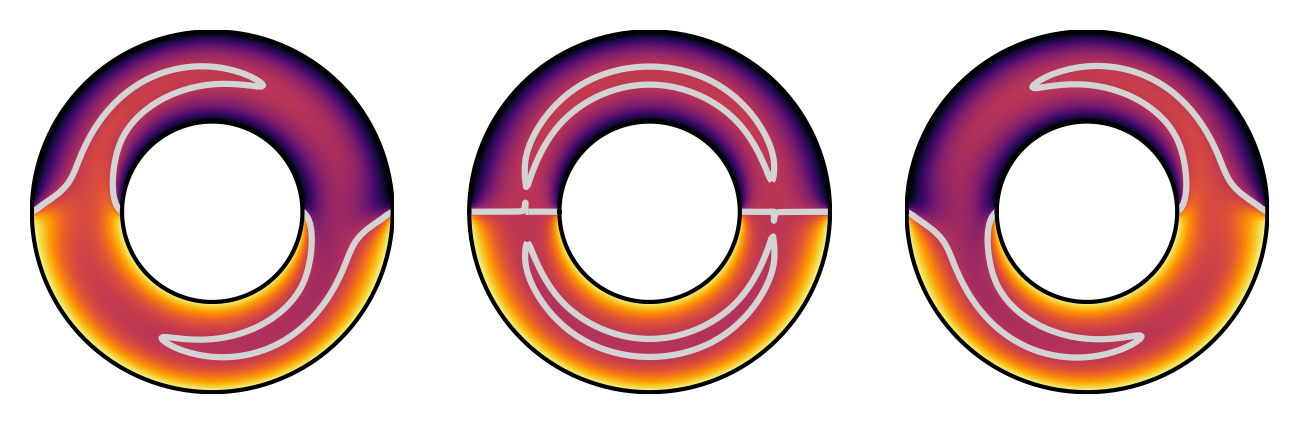
\includegraphics[width=.5\paperwidth]{cover_thermosyphon.png}}

\date[unused]{SCAI Tutorials, Jan.\ 2022}

\begin{document}

% Print the title as the first slide
\titleframe

%%%%%
%%%%%
%%%%%
%%%%%
%%%%%

\begin{frame}[t, c]{Who am I?}{}
  \begin{minipage}{.68\textwidth}
    \begin{itemize}
    \item Ma\^itre de Conférences in Fluid Dynamics (but mainly teaching Applied Mathematics).

      \medskip

    \item Machine-Learning enthusiast.

      \medskip
      
    \item Particular emphasis on the application of ML to engineering systems.
 
      \medskip
 
    \item Excited by data-efficient models with some kind of guarantees of optimality.
    \end{itemize}
  \end{minipage}%
  \hfill
  \begin{minipage}{.28\textwidth}
    \centering
    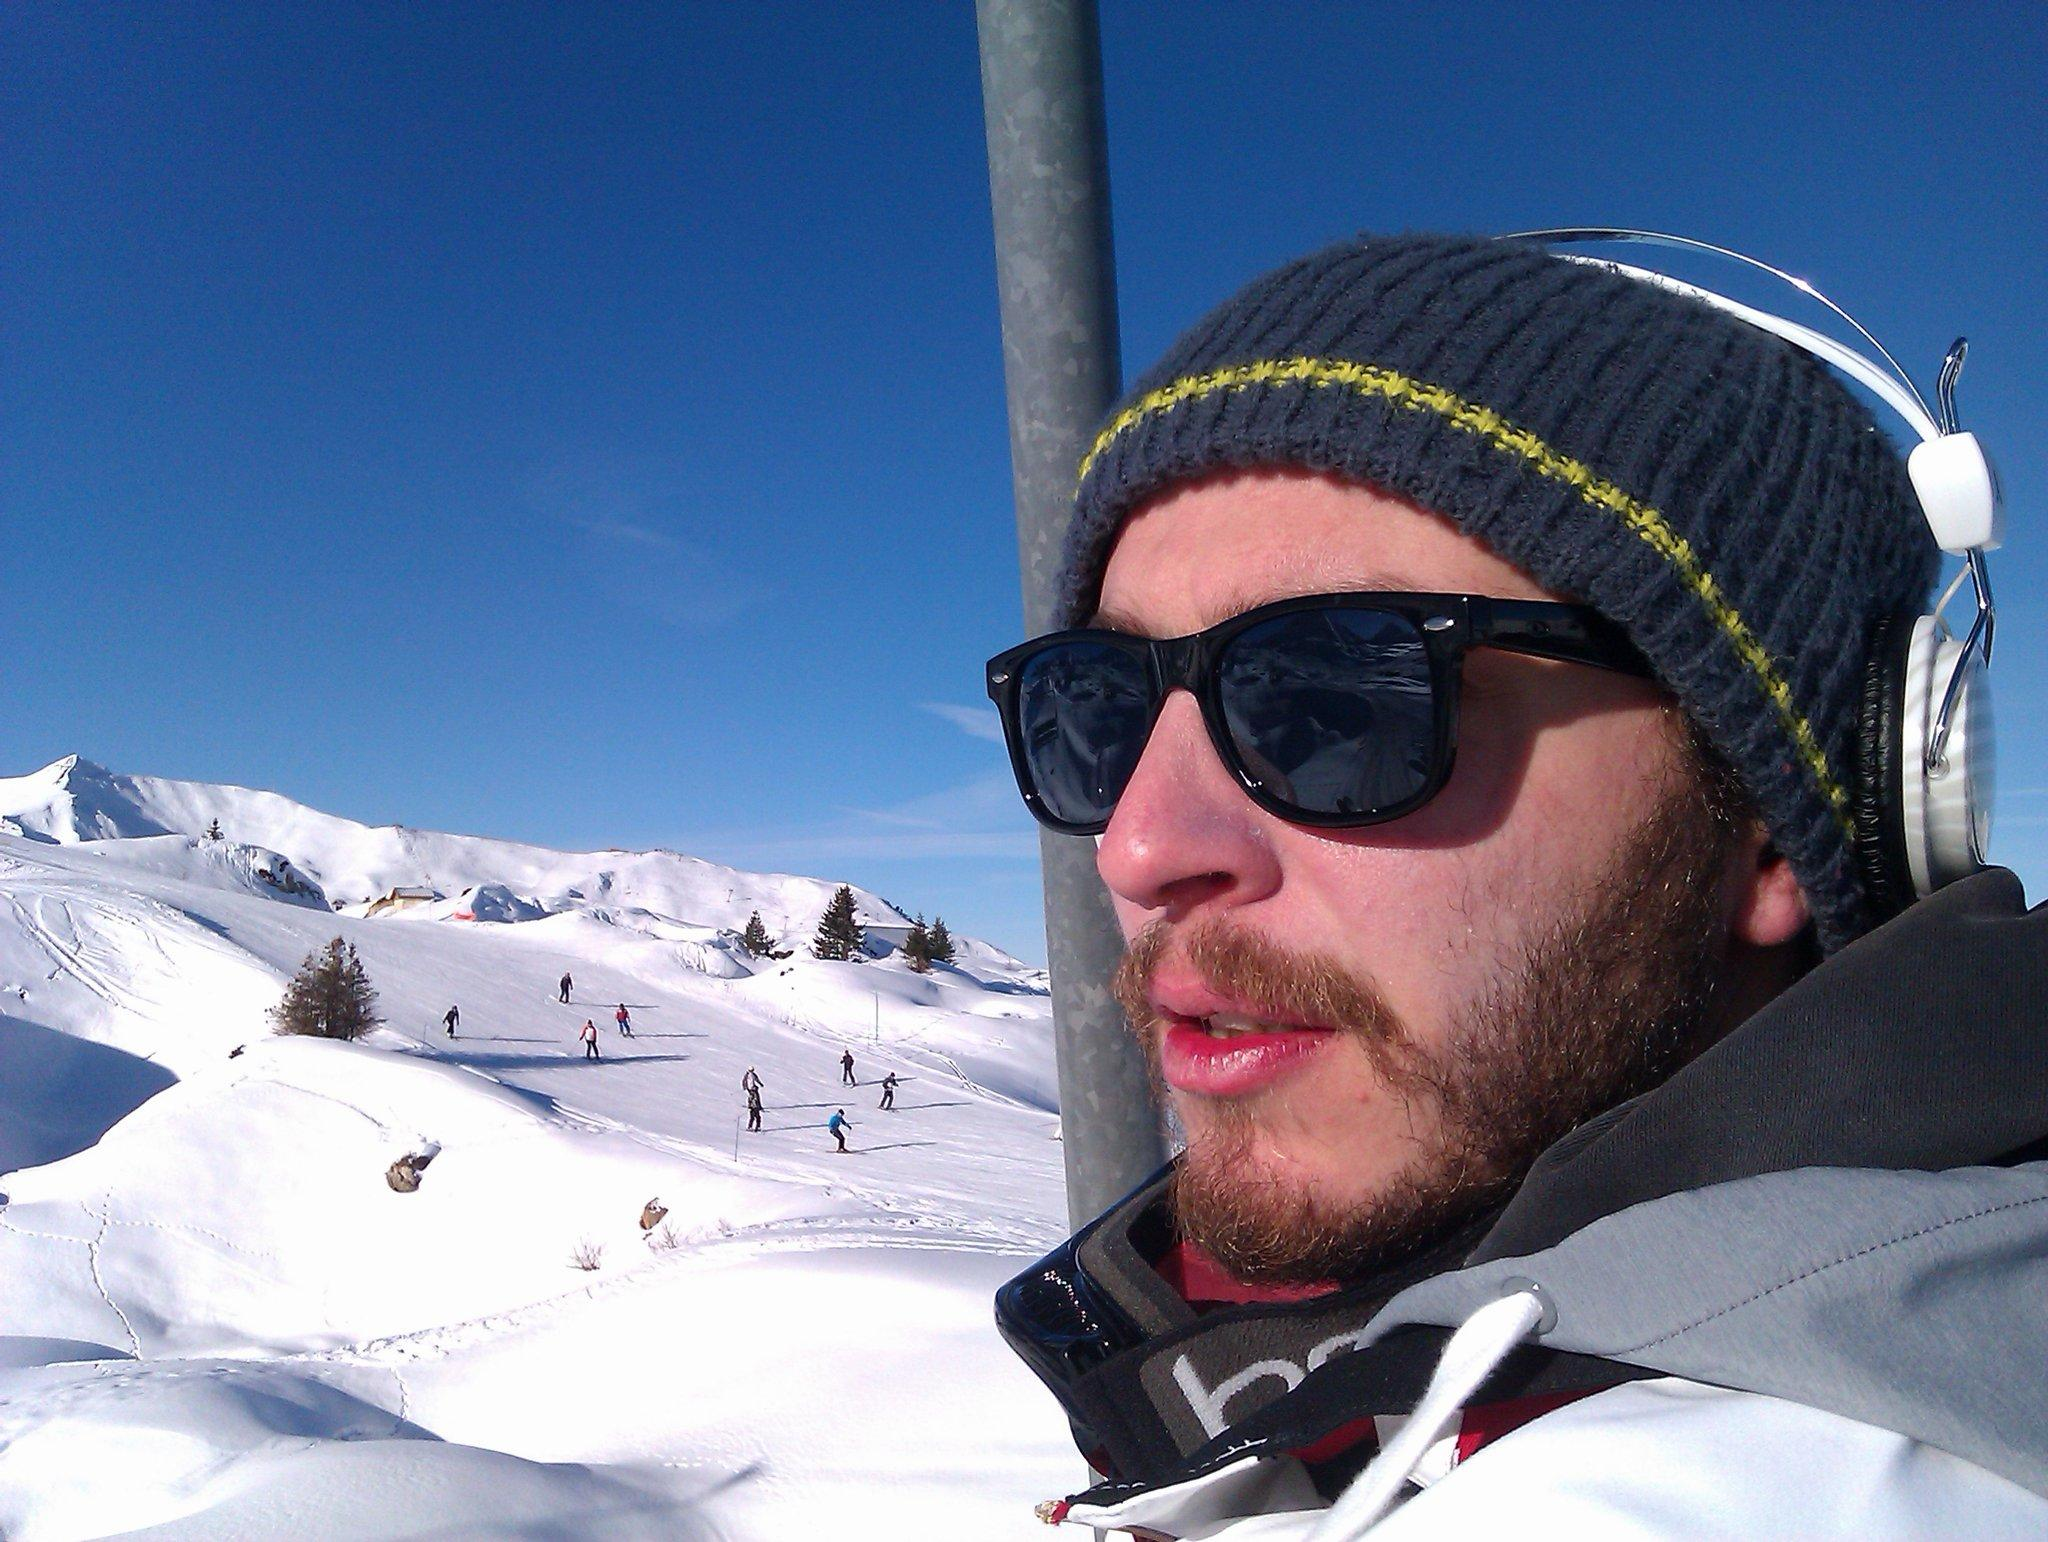
\includegraphics[width=\textwidth]{myself}
  \end{minipage}

  \vspace{1cm}
\end{frame}

%%%%%%%%%%%%%%%%%%%%%%%%%%%%%%%%
%%%%%                      %%%%%
%%%%%     INTRODUCTION     %%%%%
%%%%%                      %%%%%
%%%%%%%%%%%%%%%%%%%%%%%%%%%%%%%%

\begin{frame}[t, c]{A gallery of fluid examples}{Illustrative examples}
	\vspace{-0.5cm}
  \begin{minipage}{.64\textwidth}
    \centering
		\movie[width=\textwidth, autostart, loop]{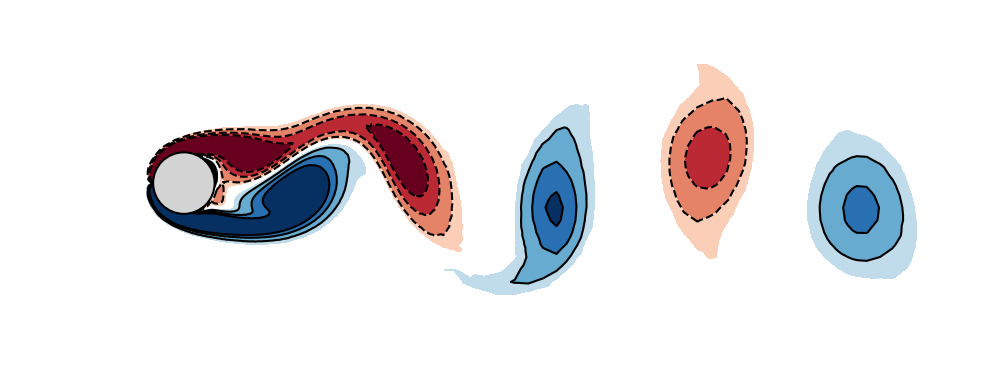
\includegraphics[width=\textwidth]{snapshot_re125_0}}{imgs/re125.mp4} \\

		Aerodynamics

		\medskip

		\movie[width=\textwidth, autostart, loop]{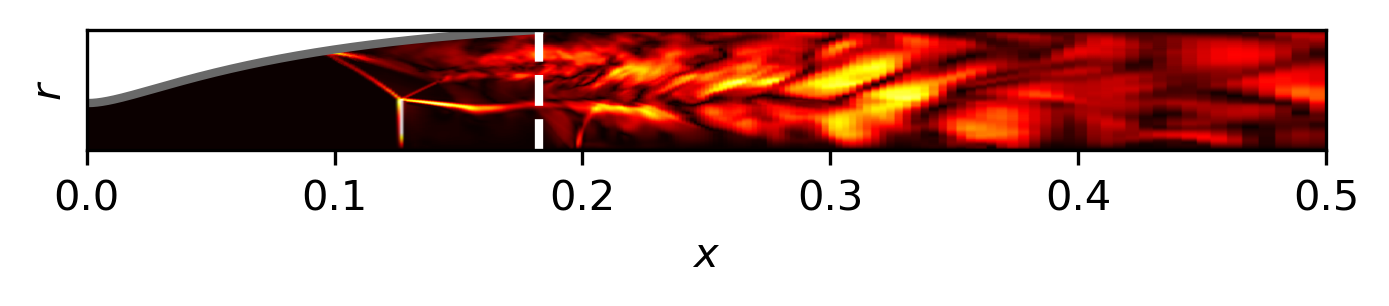
\includegraphics[width=\textwidth]{tic_m=1_fourier_mode_snapshot}}{imgs/tic_m=1_evolution.mp4} \\

		Rocket Science (litterraly!)
  \end{minipage}%
  \hfill
  \begin{minipage}{.32\textwidth}
    \centering
    \movie[width=\textwidth, autostart, loop]{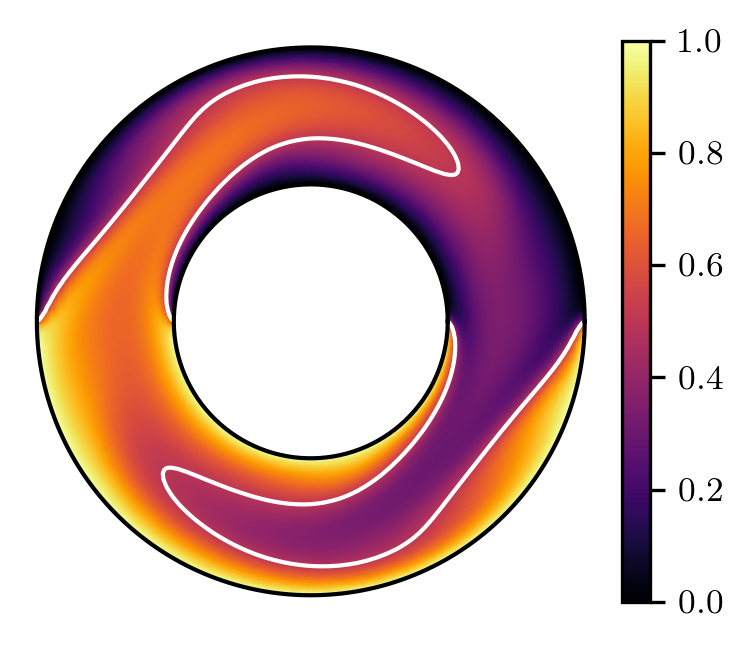
\includegraphics[width=\textwidth]{temperature_field_00000}}{imgs/temperature_evolution.mp4} \\

		Heat exchange
  \end{minipage}

\end{frame}

\begin{frame}[t, c]{A gallery of fluid examples}{Machine learning for physical systems}

	\centering
	\includegraphics[width=.8\textwidth]{physics_machine_learning}

	\vspace{1cm}
\end{frame}

\begin{frame}[t, c]{A gallery of fluid examples}{Low-order models}
	\begin{minipage}{.58\textwidth}
		\begin{itemize}
			\item Models can come in a lot of different flavors.

			\medskip

			\item Wiener proposed the following classification
			\begin{itemize}
				\item[\( \hookrightarrow	\)] \textbf{Black box:} input-output data.
				\item[\( \hookrightarrow	\)] \textbf{White box:} Input-output + known model.
				\item[\( \hookrightarrow	\)] \textbf{Gray box:} Input-output + partial knowledge of the model / inductive biases.
			\end{itemize}

			\medskip

			\item In physics, we are often in the third class.
			\begin{itemize}
				\item[\( \hookrightarrow	\)] Exact form of the equations may be unknown.
				\item[\( \hookrightarrow	\)] Knowledge of symmetries or invariants.
			\end{itemize}
		\end{itemize}
	\end{minipage}%
	\hfill
	\begin{minipage}{.38\textwidth}
		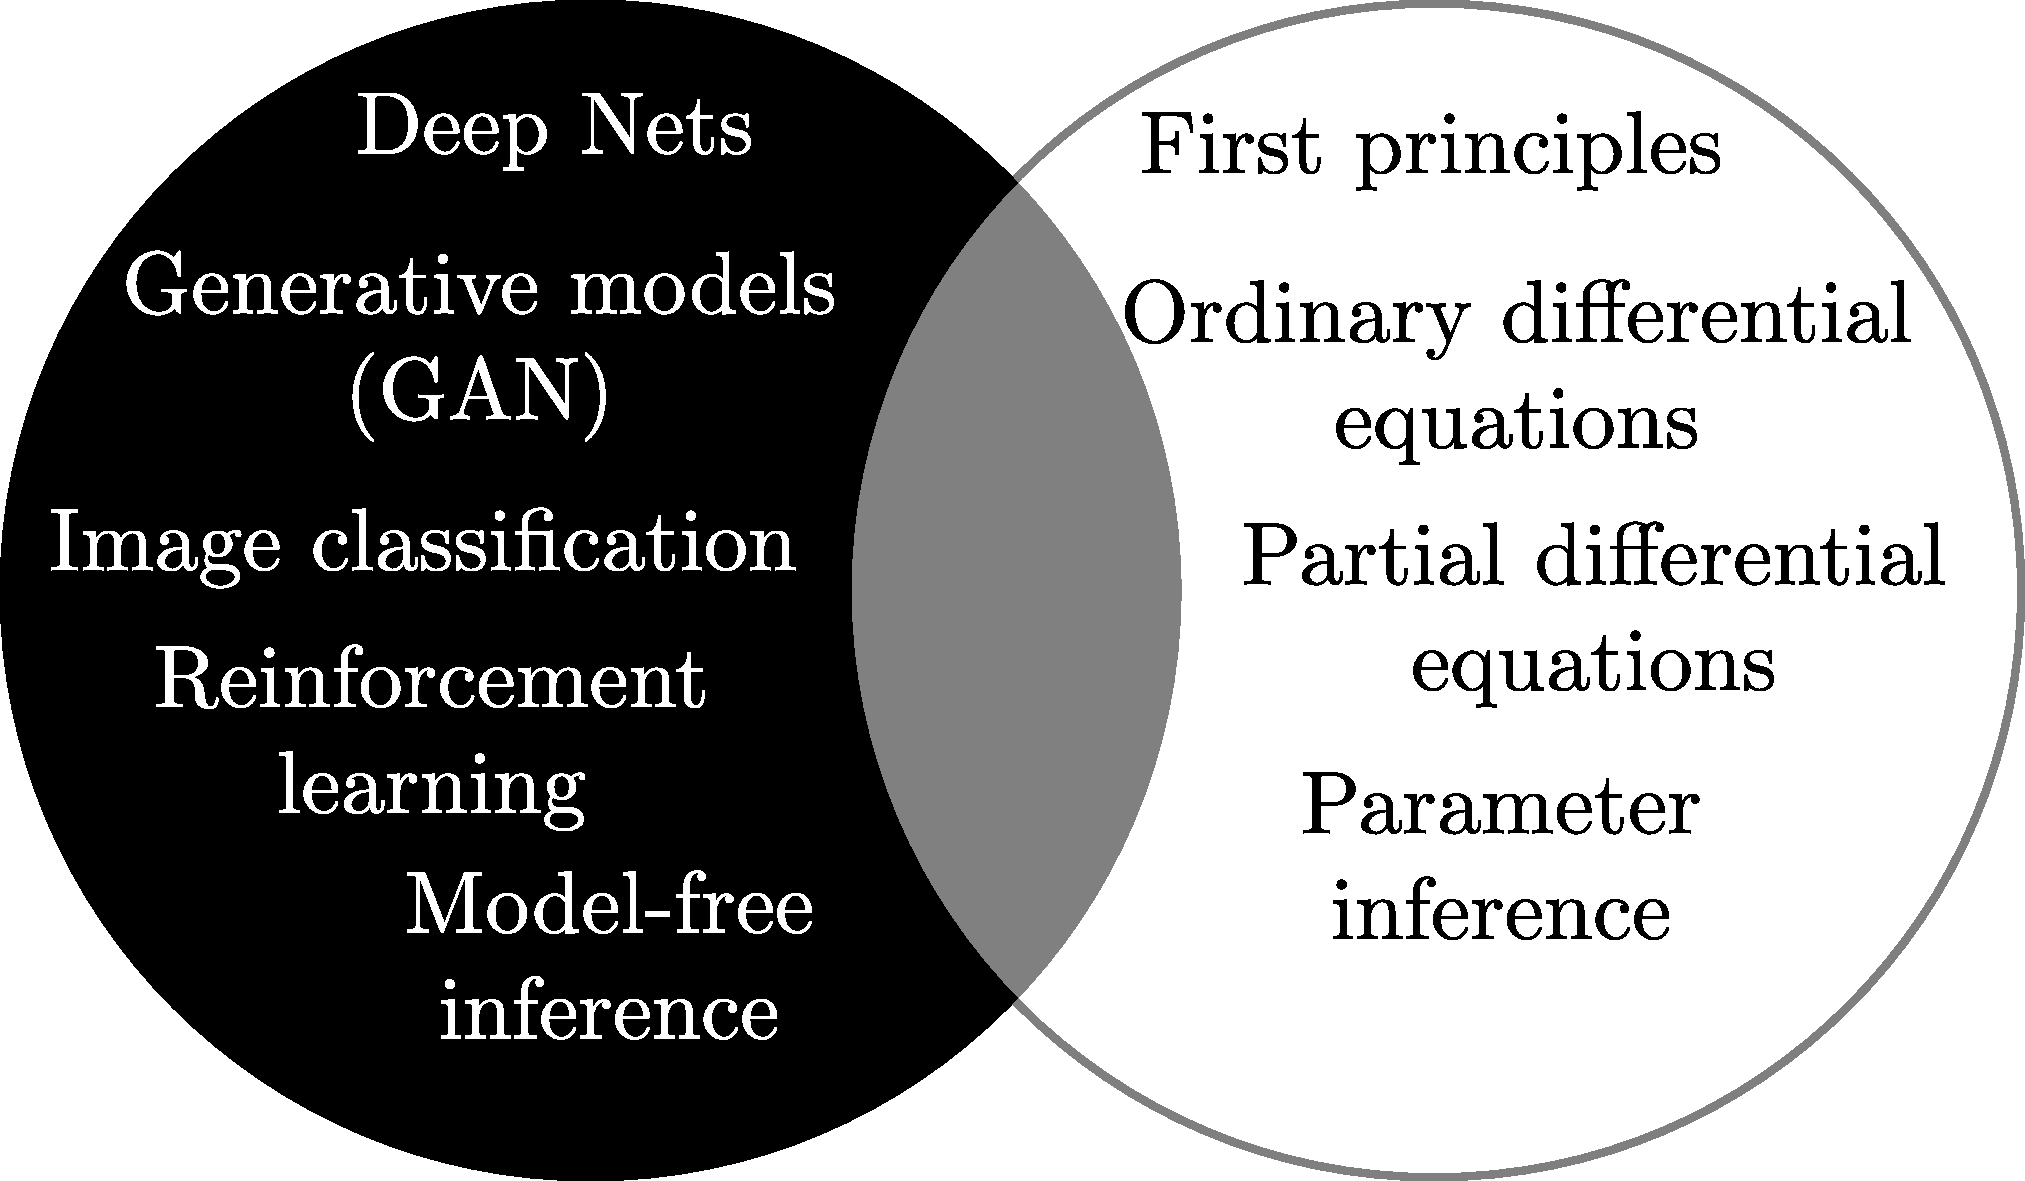
\includegraphics[width=\textwidth]{general_overview}
	\end{minipage}

	\vspace{1cm}
\end{frame}


\begin{frame}[t, c]{A gallery of fluid examples}{A prototypical example}

	\centering
	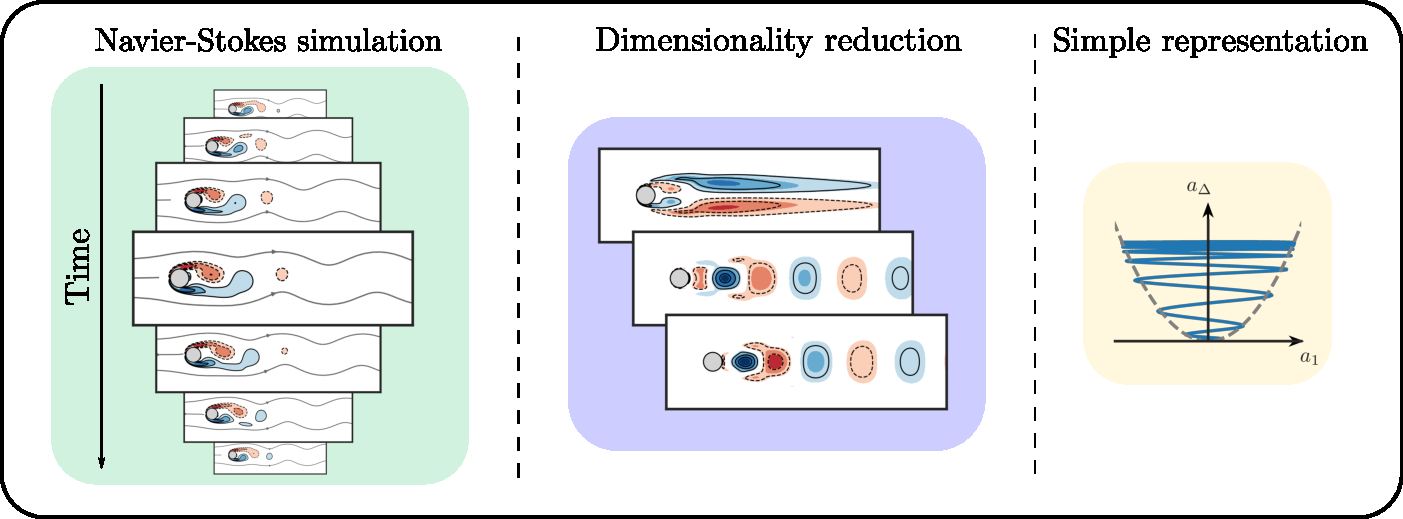
\includegraphics[width=.9\textwidth]{reduced_order_modeling}

	\vspace{1cm}
\end{frame}

\begin{frame}[t, c]{A gallery of fluid examples}{Low-order \underline{deterministic} models}
	\begin{minipage}{.58\textwidth}

		\begin{block}{}
			\textbf{Aim :} Identify an \underline{interpretable} and \underline{physically-consistent} low-order model.
		\end{block}

		\medskip

		\begin{itemize}
			\item Using \emph{SINDy}, the following model can be identified.
			%
			\[
				\begin{aligned}
					\dot{a}_1 & = \sigma a_1 - \omega a_2 - \alpha (a_1^2 + a_2^2) a_1 - \beta (a_1^2 + a_2^2) a_2 \\
					\dot{a}_2 & = \omega a_1 + \sigma a_2 + \beta (a_1^2 + a_2^2) a_1 - \alpha (a_1^2 + a_2^2) a_1.
				\end{aligned}
			\]

			\item \textbf{Interpretability :} Normal form of a supercritical Andronov-Poincaré-Hopf bifurcation.

			\item \textbf{Physical-consistency :} By design.
		\end{itemize}
	\end{minipage}%
	\hfill
	\begin{minipage}{.38\textwidth}
		\centering
		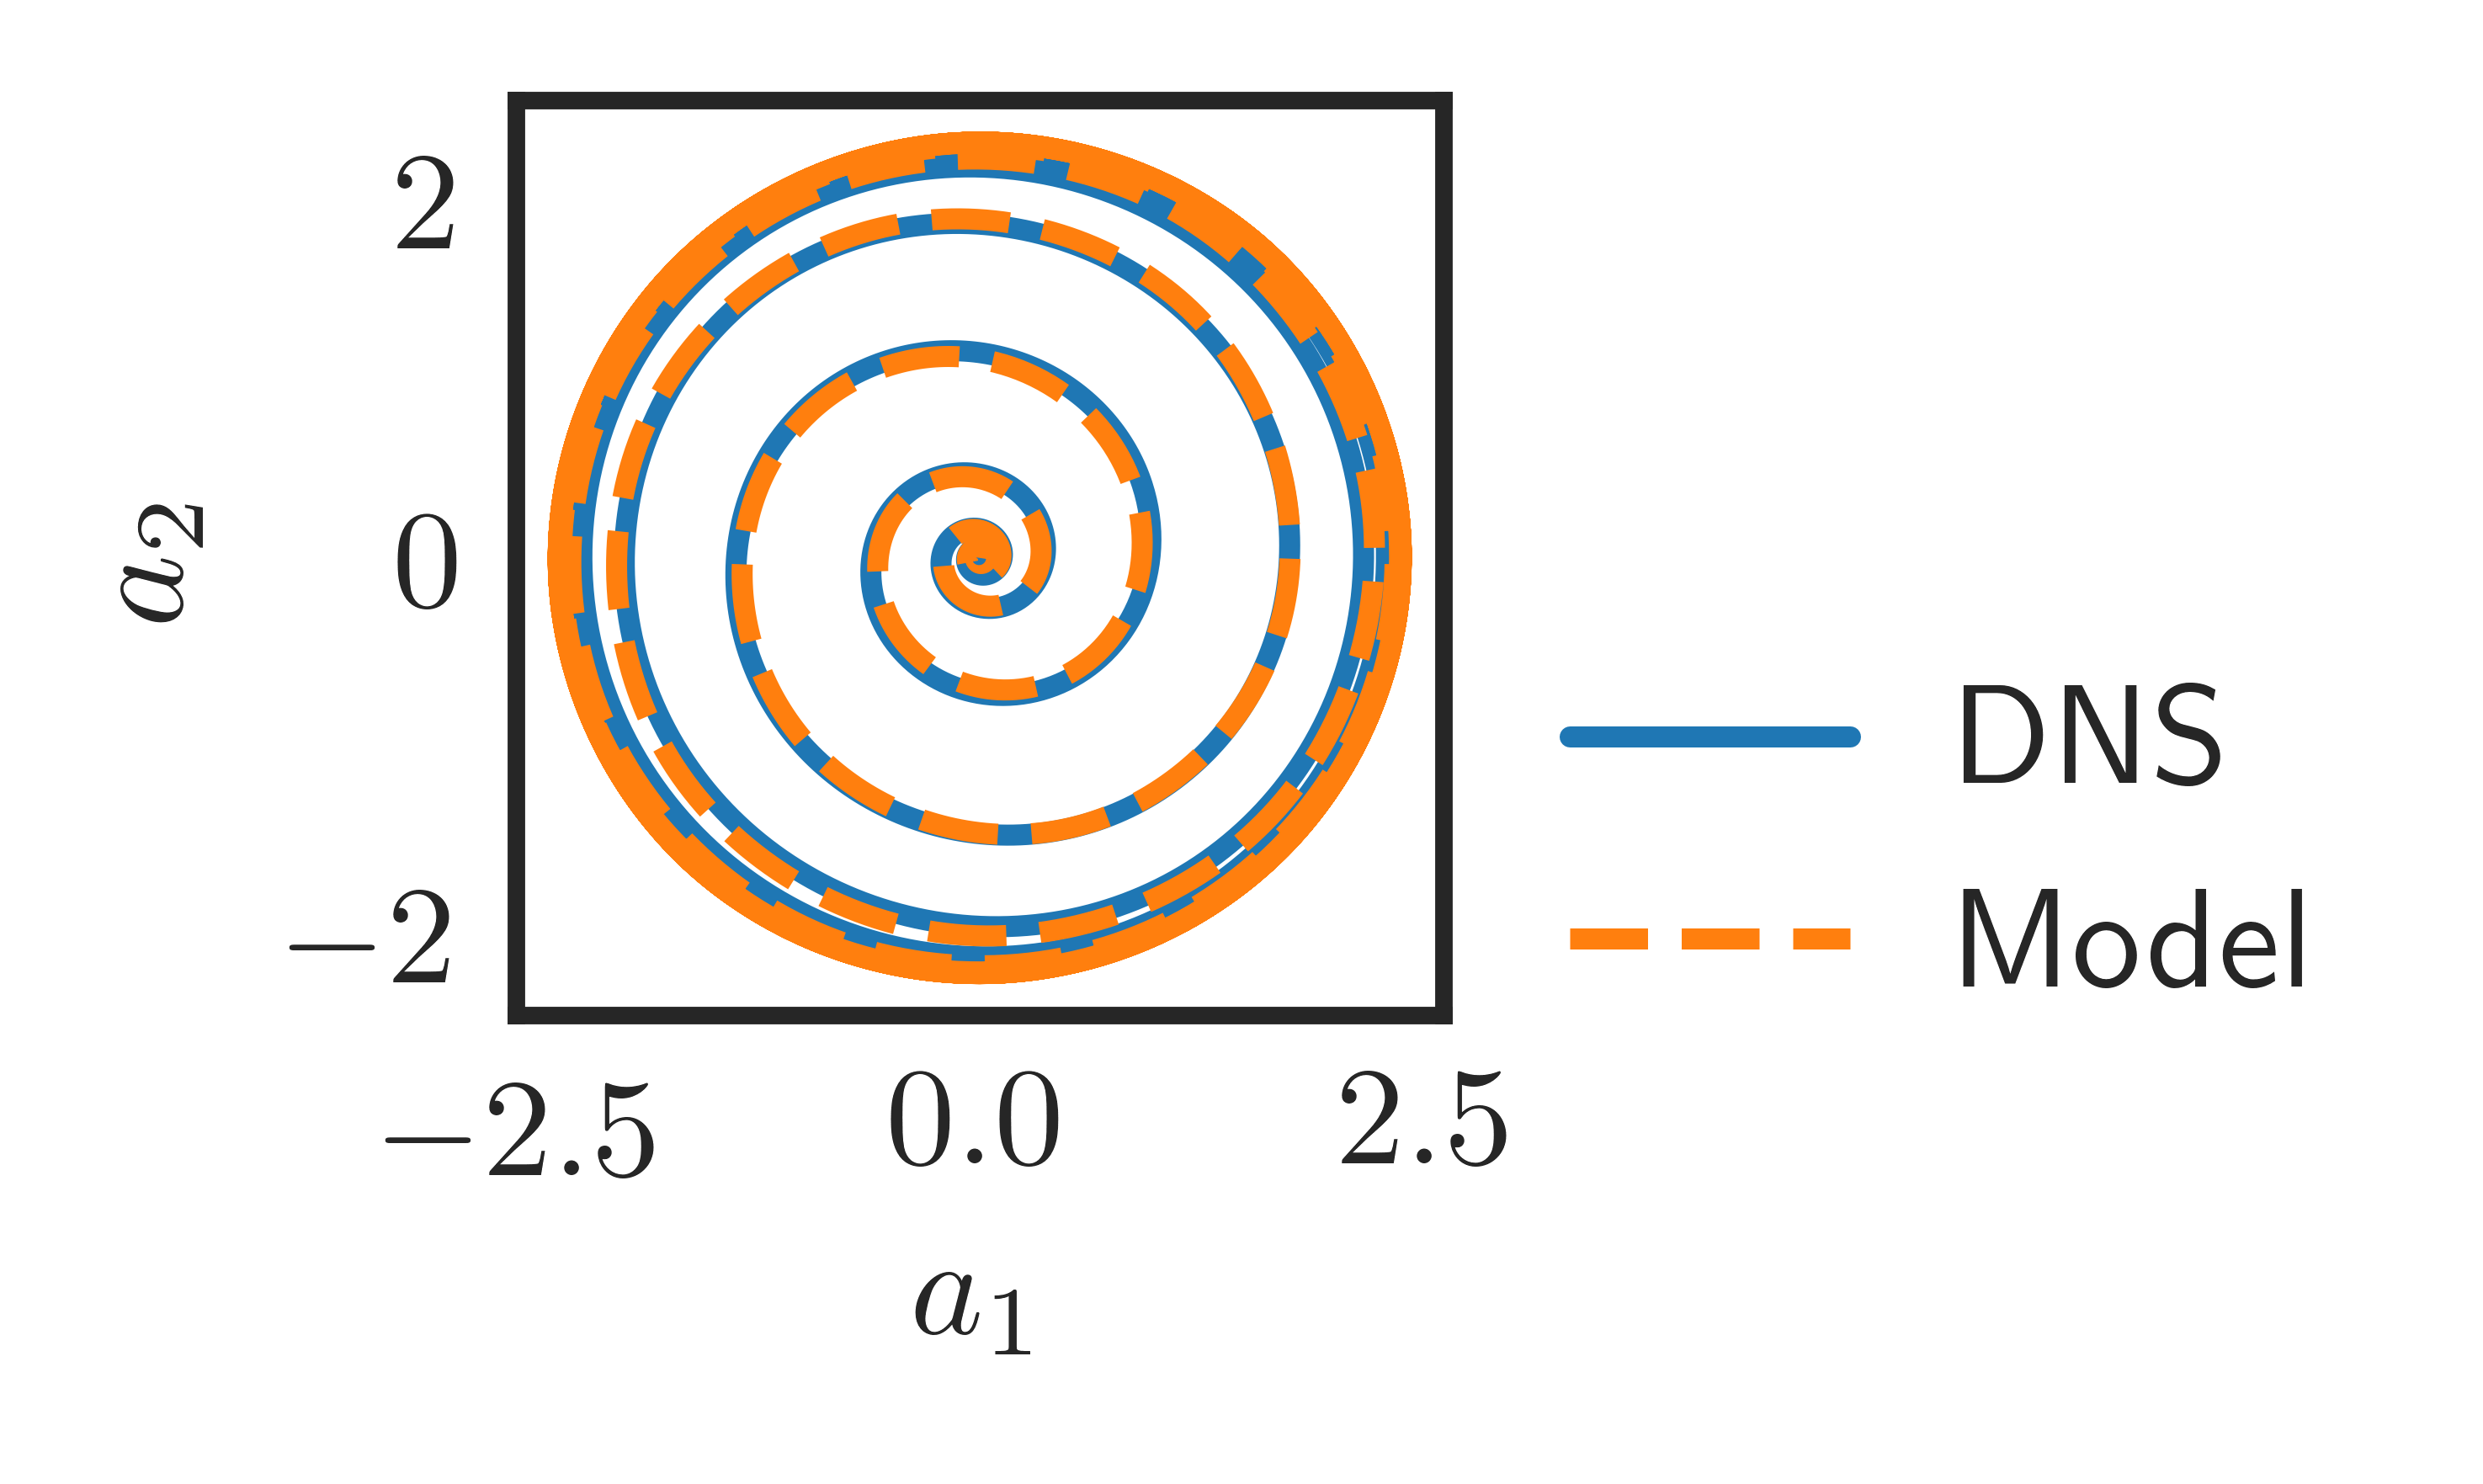
\includegraphics[width=\textwidth]{low_dimensional_phase_plot}
	\end{minipage}

	\vspace{1cm}
\end{frame}

\begin{frame}[t, c]{A gallery of fluid examples}{Low-order \underline{probabilistic} models}
	\begin{minipage}{.38\textwidth}
		\begin{tikzpicture}
			\node[state] (s1) {\( \bm{s}_1 \)};
			\node[state, below right of=s1] (s2) {\( \bm{s}_2 \)};
			\node[state, below left of=s1] (s4) {\( \bm{s}_4 \)};
			\node[state, below left of=s2] (s3) {\( \bm{s}_3 \)};

			\draw (s1) edge[loop above] node {\(l_{11}\)} (s1);
			\draw (s1) edge[bend left] node {\(l_{21}\)}  (s2);

			\draw (s2) edge[loop right]  node {\(l_{22}\)} (s2);
			\draw (s2) edge[bend left]  node {\(l_{32}\)} (s3);

			\draw (s3) edge[bend left]  node {\(l_{43}\)} (s4);
			\draw (s3) edge[loop below]  node {\(l_{33}\)} (s3);

			\draw (s4) edge[bend left]  node {\(l_{14}\)} (s1);
			\draw (s4) edge[loop left]  node {\(l_{44}\)} (s4);

		\end{tikzpicture}
	\end{minipage}%
	\hfill
	\begin{minipage}{.58\textwidth}
		\begin{block}{}
			\centering
			\textbf{Aim :} Identify a \underline{coarse-grain probabilistic} low-order model.
		\end{block}

		\medskip

		\begin{itemize}
			\item Using clustering and symbolic dynamics, a discrete-time probabilistic model can be identified.
			%
			\[
				\bm{p}_{k+1} = \bm{L} \bm{p}_k.
			\]

			\item \textbf{Interpretability :} \( \bm{L} \) describes the transition probability between discrete states \( \bm{s}_i \).

			\medskip

			\item Dynamics are encoded as a probabilistic \underline{finite state machine}.
		\end{itemize}
	\end{minipage}

	\vspace{1cm}
\end{frame}

\begin{frame}[t, c]{Low-order modeling}{Ideal setup}

	\centering

	\begin{tikzpicture}
   	% \draw[help lines](0,0) grid (10,5);

		\node[fill=blue!20, minimum width=1cm, minimum height=3cm, rounded corners, draw=black, thick] (X) at (0, 2.5) {\( \bm{q}_k \)};

		\draw[fill=gray!10, thick] ([xshift=0.75cm]X.north east) -- ([xshift=2.75cm,yshift=0.5cm]X.east) -- ([xshift=2.75cm,yshift=-0.5cm]X.east) -- ([xshift=0.75cm]X.south east) -- cycle;
		\node at (2.25, 2.5) {\textsc{Encoder}};

		\node[fill=gray!10, minimum width=2cm, minimum height=1.0cm, rounded corners, thick, draw=black] (Z) at (5cm, 2.5) {\( \dot{\bm{x}} = \bm{f}(\bm{x}) \)};
		\node at (5, 3.333) {\textsc{Dynamics}};

		\draw[fill=gray!10, thick] ([xshift=0.75cm]Z.north east) -- ([xshift=2.75cm,yshift=1cm]Z.north east) -- ([xshift=2.75cm,yshift=-1cm]Z.south east) -- ([xshift=0.75cm]Z.south east) -- cycle;
		\node at (7.75, 2.5) {\textsc{Decoder}};

		\node[fill=blue!20, minimum width=1cm, minimum height=3cm, rounded corners, draw=black, thick] (Xp) at (10, 2.5) {\( \bm{q}_{k+1} \)};

		\draw[arrow] (X.east) -- ([xshift=0.75cm]X.east);
		\draw[arrow] ([xshift=-0.75cm]Z.west) -- (Z.west);
		\draw[arrow] (Z.east) -- ([xshift=0.75cm]Z.east);
		\draw[arrow] ([xshift=-0.75cm]Xp.west) -- (Xp.west);

	\end{tikzpicture}

	\bigskip

	\begin{block}{}
		\textbf{Ideal setup :} Learn jointly the encoding from the high-dimensional space to the low-dimensional one and the dynamical model within this subspace.
	\end{block}

	\vspace{1cm}
\end{frame}

\begin{frame}[t, c]{Low-order modeling}{In practice}

	\centering

	\begin{tikzpicture}
   	% \draw[help lines](0,0) grid (10,5);

		\node[fill=blue!20, minimum width=1cm, minimum height=3cm, rounded corners, draw=black, thick] (X) at (0, 2.5) {\( \bm{q}_k \)};

		\draw[fill=gray!10, thick] ([xshift=0.75cm]X.north east) -- ([xshift=2.75cm,yshift=0.5cm]X.east) -- ([xshift=2.75cm,yshift=-0.5cm]X.east) -- ([xshift=0.75cm]X.south east) -- cycle;
		\node at (2.25, 2.5) {\textsc{Encoder}};

		\node[fill=gray!10, minimum width=2cm, minimum height=1.0cm, rounded corners, thick, draw=black] (Z) at (5cm, 2.5) {\( \dot{\bm{x}} = \bm{f}(\bm{x}) \)};
		\node at (5, 3.333) {\textsc{Dynamics}};

		\draw[fill=gray!10, thick] ([xshift=0.75cm]Z.north east) -- ([xshift=2.75cm,yshift=1cm]Z.north east) -- ([xshift=2.75cm,yshift=-1cm]Z.south east) -- ([xshift=0.75cm]Z.south east) -- cycle;
		\node at (7.75, 2.5) {\textsc{Decoder}};

		\node[fill=blue!20, minimum width=1cm, minimum height=3cm, rounded corners, draw=black, thick] (Xp) at (10, 2.5) {\( \bm{q}_{k+1} \)};

		\draw[arrow] (X.east) -- ([xshift=0.75cm]X.east);
		\draw[arrow] ([xshift=-0.75cm]Z.west) -- (Z.west);
		\draw[arrow] (Z.east) -- ([xshift=0.75cm]Z.east);
		\draw[arrow] ([xshift=-0.75cm]Xp.west) -- (Xp.west);

	\end{tikzpicture}

	\bigskip

	\begin{block}{}
		\textbf{In practice :} Learning jointly the encoder/decoder and the dynamical model is complicated.
		In practice, they are learned sequentially (i.e.\ first encoder/decoder and then the dynamical model).
	\end{block}

	\vspace{1cm}
\end{frame}

\begin{frame}[t, c]{Our setup for today}{2D Thermosiphon}
  \begin{minipage}{.58\textwidth}
    \begin{itemize}
      \item Two-dimensional flow governed by the incompressible Navier-Stokes equations
      %
      \[
      \begin{aligned}
        \frac{\partial \bm{u}}{\partial t} + (\bm{u} \cdot \nabla ) \bm{u} & = -\nabla p + \textrm{Pr} \nabla^2 \bm{u} + \textrm{Ra Pr } \boldsymbol{\theta} \bm{e}_y \\
        \frac{\partial \boldsymbol{\theta}}{\partial t} + \left( \bm{u} \cdot \nabla \right) \boldsymbol{\theta} & = \nabla^2 \boldsymbol{\theta}.
      \end{aligned}
      \]

      \item \(  Ra  \) and \( Pr  \) are parameters defining our problem.
      \begin{itemize}
        \item[\(  \hookrightarrow \)] \(  Ra  \)   is set to \( Ra = 17\ 000  \).
        \item[\(  \hookrightarrow \)] \(  Pr  \) is set to \( Pr = 5 \).
      \end{itemize}
    \end{itemize}
  \end{minipage}%
  \hfill
  \begin{minipage}{.38\textwidth}
    \centering
    \movie[width=\textwidth, autostart, loop]{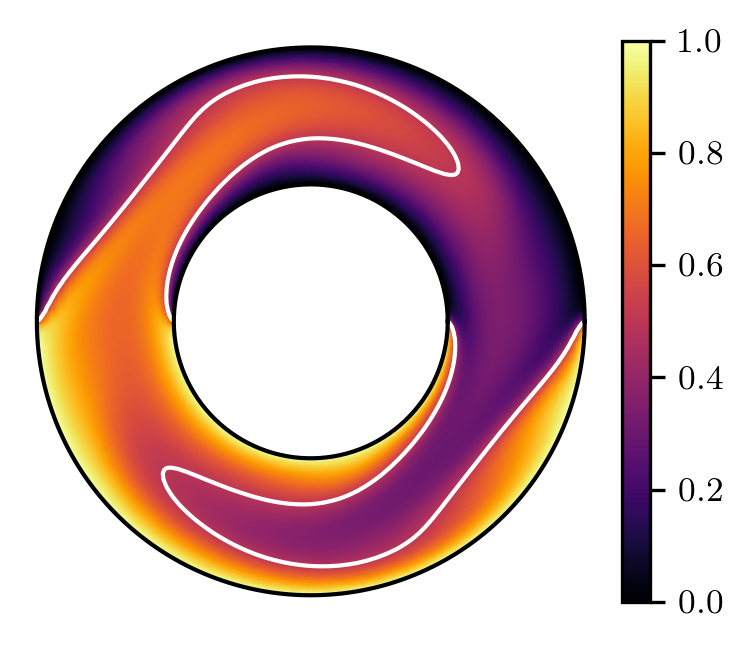
\includegraphics[width=\textwidth]{temperature_field_00000}}{imgs/temperature_evolution.mp4} \\
    {\small
    \textbf{Fig:} Chaotic thermosyphon temp.\ field.
    }
  \end{minipage}

  \vspace{1cm}
\end{frame}

% \begin{frame}[t, c]{2D Thermosiphon}{Chaotic dynamics}
%   \centering
%   % 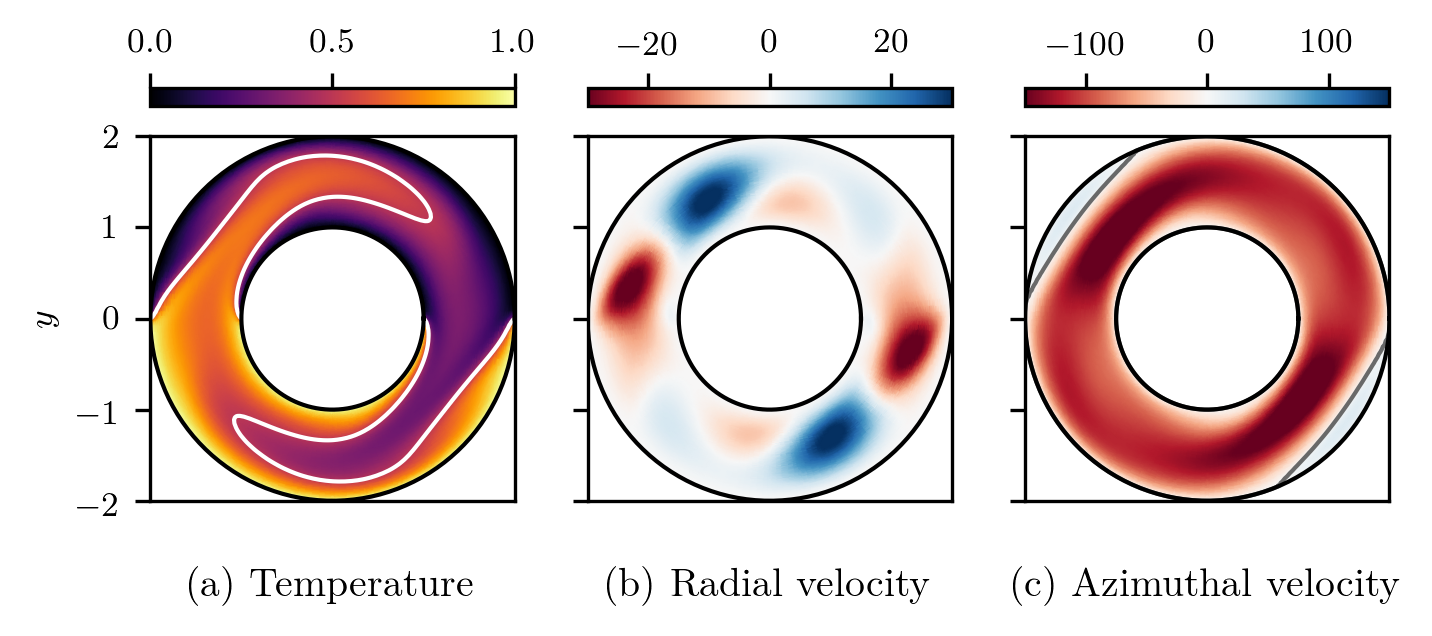
\includegraphics[width=.9\textwidth]{chaotic_thermosyphon_00000}
%   \movie[width=.9\textwidth, autostart, loop]{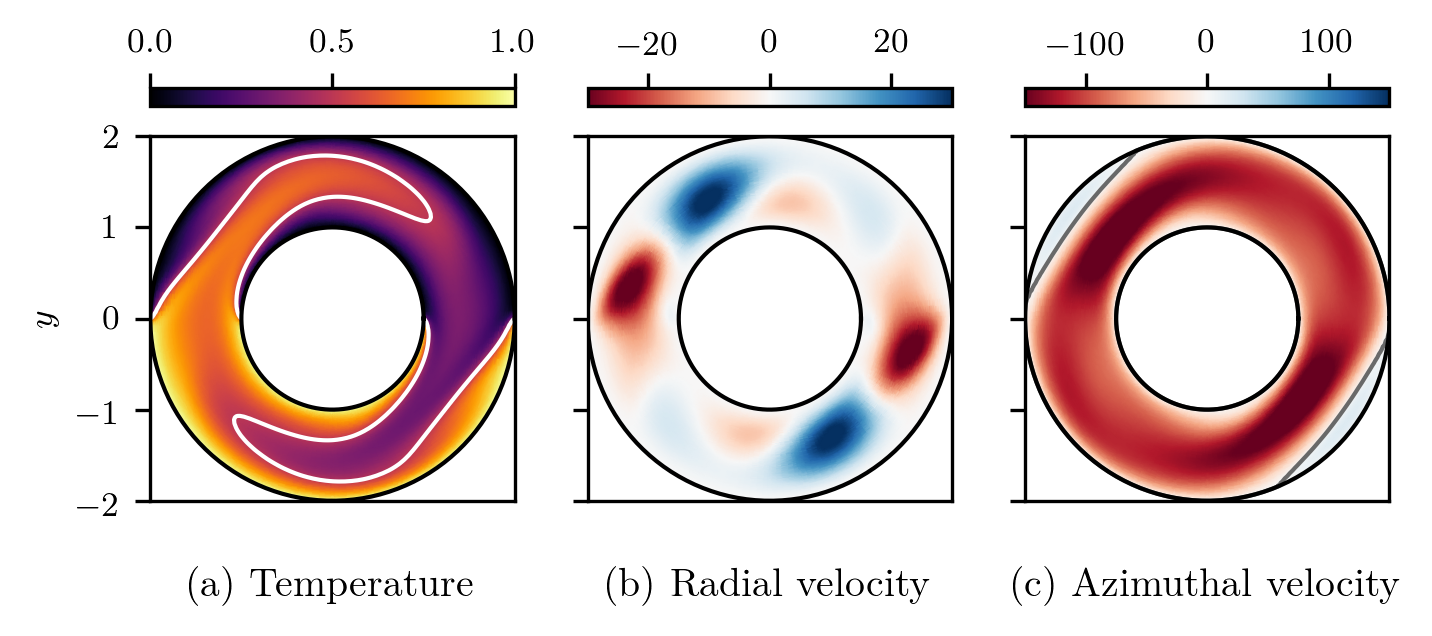
\includegraphics[width=.9\textwidth]{chaotic_thermosyphon_00000}}{imgs/chaotic_thermosyphon.mp4} \\
%
%   \vspace{1cm}
% \end{frame}

\begin{frame}[t, c]{Our setup for today}{Chaotic dynamics}
		\centering
		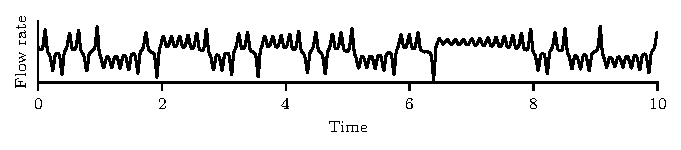
\includegraphics[width=.9\textwidth]{flow_rate_time_series}

		\begin{itemize}
			\item Time-evolution of the cross-sectional flow rate is indicative of Lorenz-like chaotic dynamics.
			\begin{itemize}
				\item[\(	\hookrightarrow	\)] "Random" switching between clockwise and anti-clockwise rotation.
			\end{itemize}

			\medskip

			\item \underline{\textbf{Hypothesis}}: These dynamics can be captured by a low-order model.
		\end{itemize}
  \vspace{1cm}
\end{frame}

\begin{frame}[t, c]{Our setup for today}{A quick detour}
	\begin{minipage}{.58\textwidth}
		\begin{itemize}
			\item Most notorious chaotic dynamical system proposed by Edward Lorenz in 1963.
			It reads
			%
			\[
				\begin{aligned}
					\dot{x} & = \sigma \left( y - x \right) \\
					\dot{y} & = \rho x - y - xz \\
					\dot{z} & = xy - \beta z.
				\end{aligned}
			\]

			\medskip

			\item It can be derived (under certain conditions) directly from the Navier-Stokes equations.
		\end{itemize}
	\end{minipage}%
	\hfill
	\begin{minipage}{.38\textwidth}
		\movie[width=\textwidth, autostart, loop]{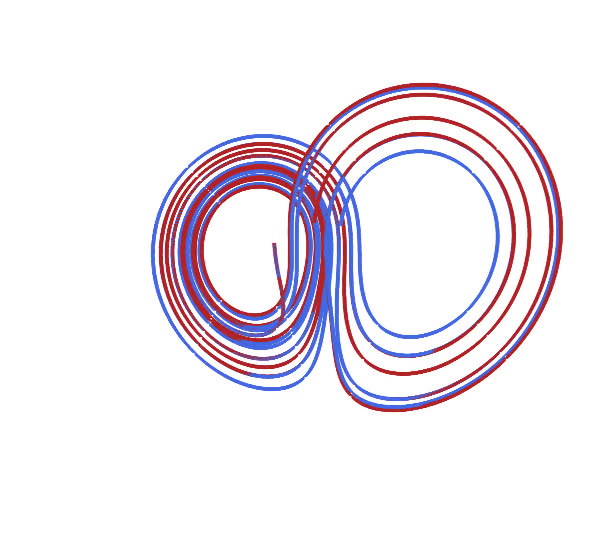
\includegraphics[width=\textwidth]{image_video_lorenz}}{imgs/Lorenz_attractor_JC.mp4}
	\end{minipage}

	\vspace{1cm}
\end{frame}

\begin{frame}[t, c]{Objectives}
  \begin{minipage}{.68\textwidth}
    \begin{itemize}

			\item What physical properties should our reduced-order model have?
			\begin{itemize}
				\item[\(	\hookrightarrow	\)] Analyze the physics prior to modeling.
			\end{itemize}

			\medskip

      \item How to obtain a good low-dimensional embedding?
      \begin{itemize}
        \item[\(  \hookrightarrow \)] Dimensionality reduction.
      \end{itemize}

      \medskip

      \item Can we identify the equations governing the dynamics in the embedded space?
      \begin{itemize}
        \item[\(  \hookrightarrow	\)] System identification.
				\item[\(	\hookrightarrow	\)] How to enforce the physical constraints?
      \end{itemize}

    \end{itemize}
  \end{minipage}%
  \hfill
  \begin{minipage}{.28\textwidth}
		\centering
		
\includegraphics[width=.8\textwidth]{objectives}
  \end{minipage}

  \vspace{1cm}
\end{frame}


%%%%%
%%%%%
%%%%%
%%%%%
%%%%%

\begin{frame}[t, c]{Chaotic thermosyphon}{Characterizing its dynamics}
  \centering
  \movie[width=.8\textwidth, autostart, loop]{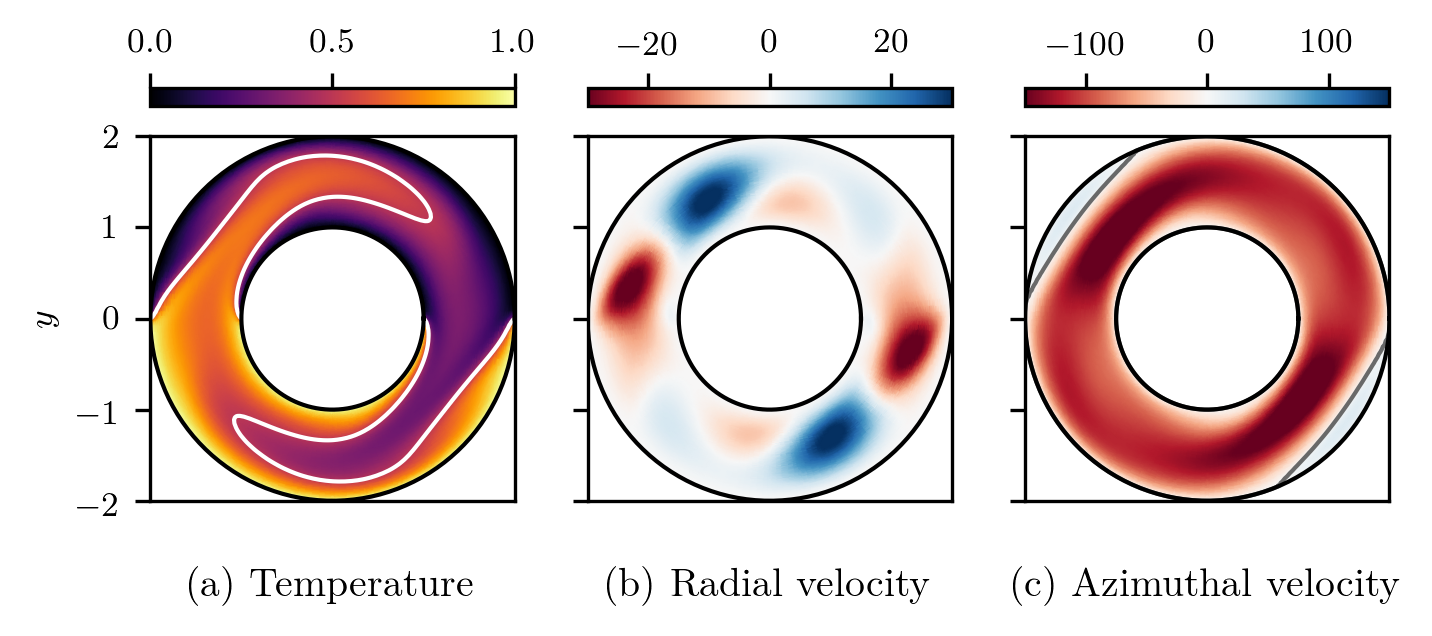
\includegraphics[width=.8\textwidth]{chaotic_thermosyphon_00000}}{imgs/chaotic_thermosyphon.mp4}

  \vspace{1cm}
\end{frame}

% \begin{frame}[t, c]{Chaotic thermosyphon}{Characterizing its dynamics}
%   \begin{minipage}{.48\textwidth}
%     \begin{itemize}
%       \item Mean flow and fluctuations are symmetric w.r.t.\ the vertical axis.
%
%       \medskip
%
%       \item Temperature fluctuations are localized close to the discontinuity at the walls.
%
%       \medskip
%
%       \item Azimuthal velocity is relatively invariant in the azimuthal direction.
%     \end{itemize}
%   \end{minipage}%
%   \hfill
%   \begin{minipage}{.48\textwidth}
%     \centering
%     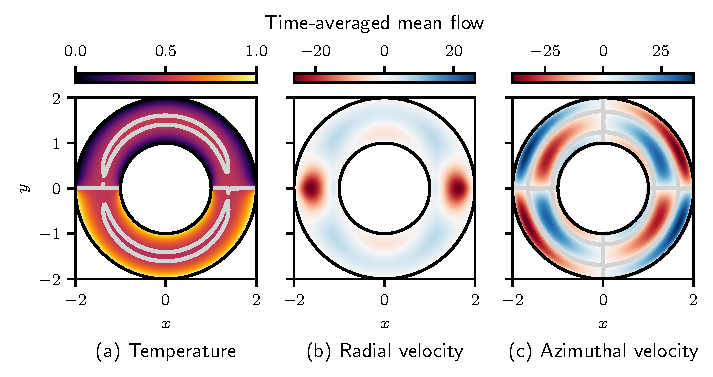
\includegraphics[width=.9\textwidth]{mean_flow} \\
%     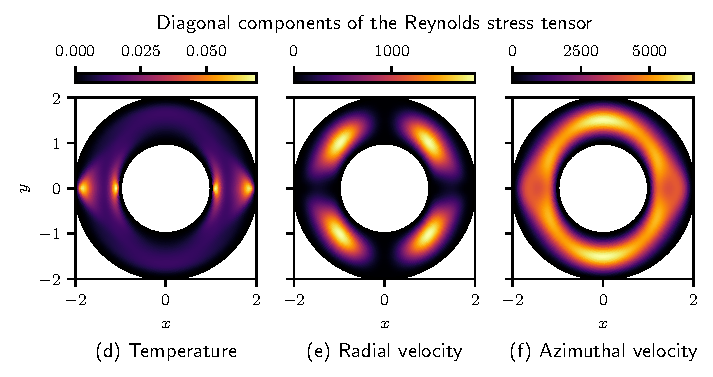
\includegraphics[width=.9\textwidth]{reynolds_stresses}
%   \end{minipage}
%
%   \vspace{1cm}
% \end{frame}

\begin{frame}[t, c]{Chaotic thermosyphon}{Characterizing its dynamics}
  \begin{minipage}{.58\textwidth}
    \begin{figure}
      \subfigure[Flow rate \( m(t) \)]{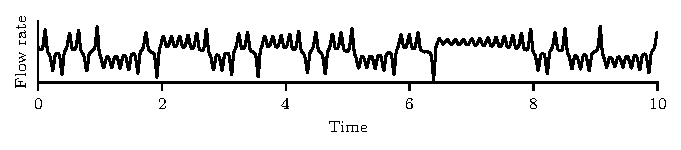
\includegraphics[width=\textwidth]{flow_rate_time_series}} \\
      \subfigure[Empirical PDF]{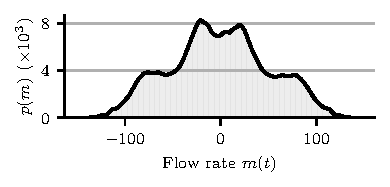
\includegraphics[width=.48\textwidth]{flow_rate_empirical_pdf}}%
      \hfill
      \subfigure[PSD of \( \dot{m}(t) \)]{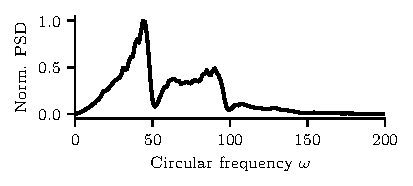
\includegraphics[width=.48\textwidth]{flow_rate_psd}}
    \end{figure}
  \end{minipage}%
  \hfill
  \begin{minipage}{.38\textwidth}
    \begin{itemize}
    \item Clockwise and counter-clockwise rotations are equally likely.

      \medskip
      
    \item Dominant time-scale associated w/ the oscillation in one direction.
      
      \medskip
      
    \item Continuous spectrum due to the chaotic nature of the system.
    \end{itemize}
  \end{minipage}

  \vspace{1cm}
\end{frame}

\begin{frame}[t, c]{Chaotic thermosyphon}{Characterizing its dynamics}
  \vspace{-0.5cm}
  % \begin{minipage}{.38\textwidth}
  %   \begin{itemize}
  %     \item Correlation decay due to the switches.

  %     \medskip

  %     \item Most of the time, a single oscillation occurs before switching.

  %     \medskip

  %     \item Behaviour very similar to that of the Lorenz system.
  %   \end{itemize}
  % \end{minipage}%
  % \hfill
  % \begin{minipage}{.58\textwidth}
    \begin{figure}
      \subfigure[Flow rate \( m(t) \)]{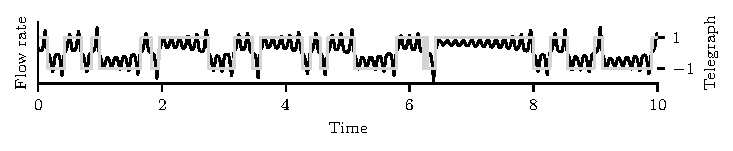
\includegraphics[width=.8\textwidth]{flow_rate_telegraph_signal}} \\
      \subfigure[Autocorr.\ function]{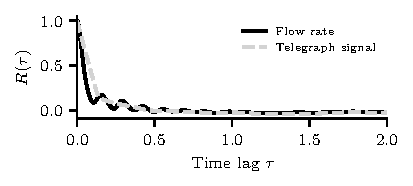
\includegraphics[width=.4\textwidth]{flow_rate_autocorrelation}}%
      %\hfill
      \subfigure[Time-scale dist.]{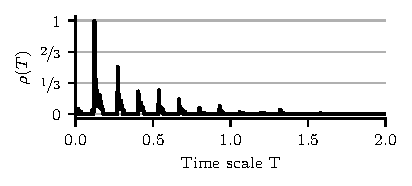
\includegraphics[width=.4\textwidth]{flow_rate_time_scale_distribution}}
    \end{figure}
  % \end{minipage}

  \vspace{2cm}
\end{frame}

% \begin{frame}[t, c]{Chaotic thermosyphon}{Connection with Lorenz system}
%   \begin{minipage}{.48\textwidth}
%     \begin{figure}
%       \centering
%       \subfigure[Lorenz time series]{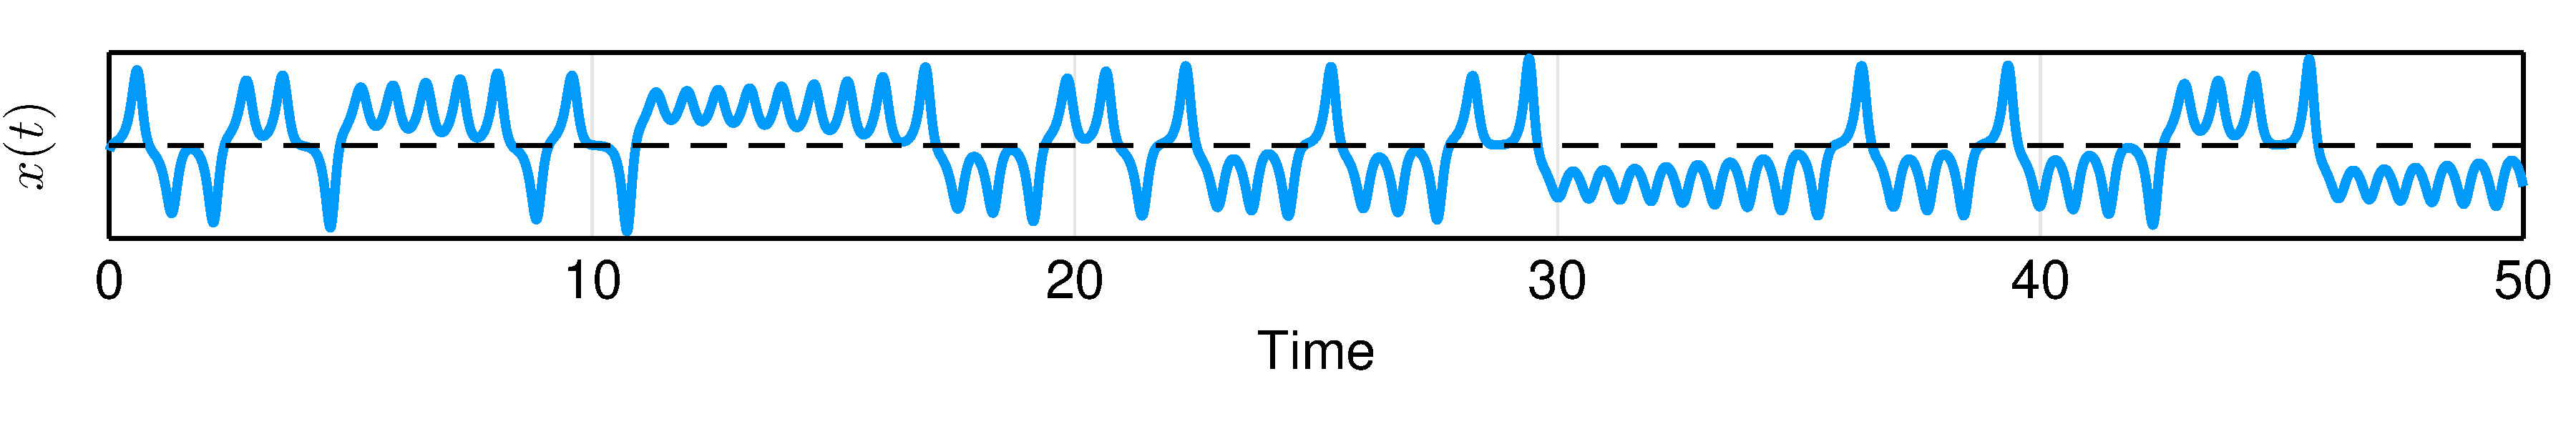
\includegraphics[width=\textwidth]{lorenz_time_series}} \\
%       \subfigure[Attractor reconstruction]{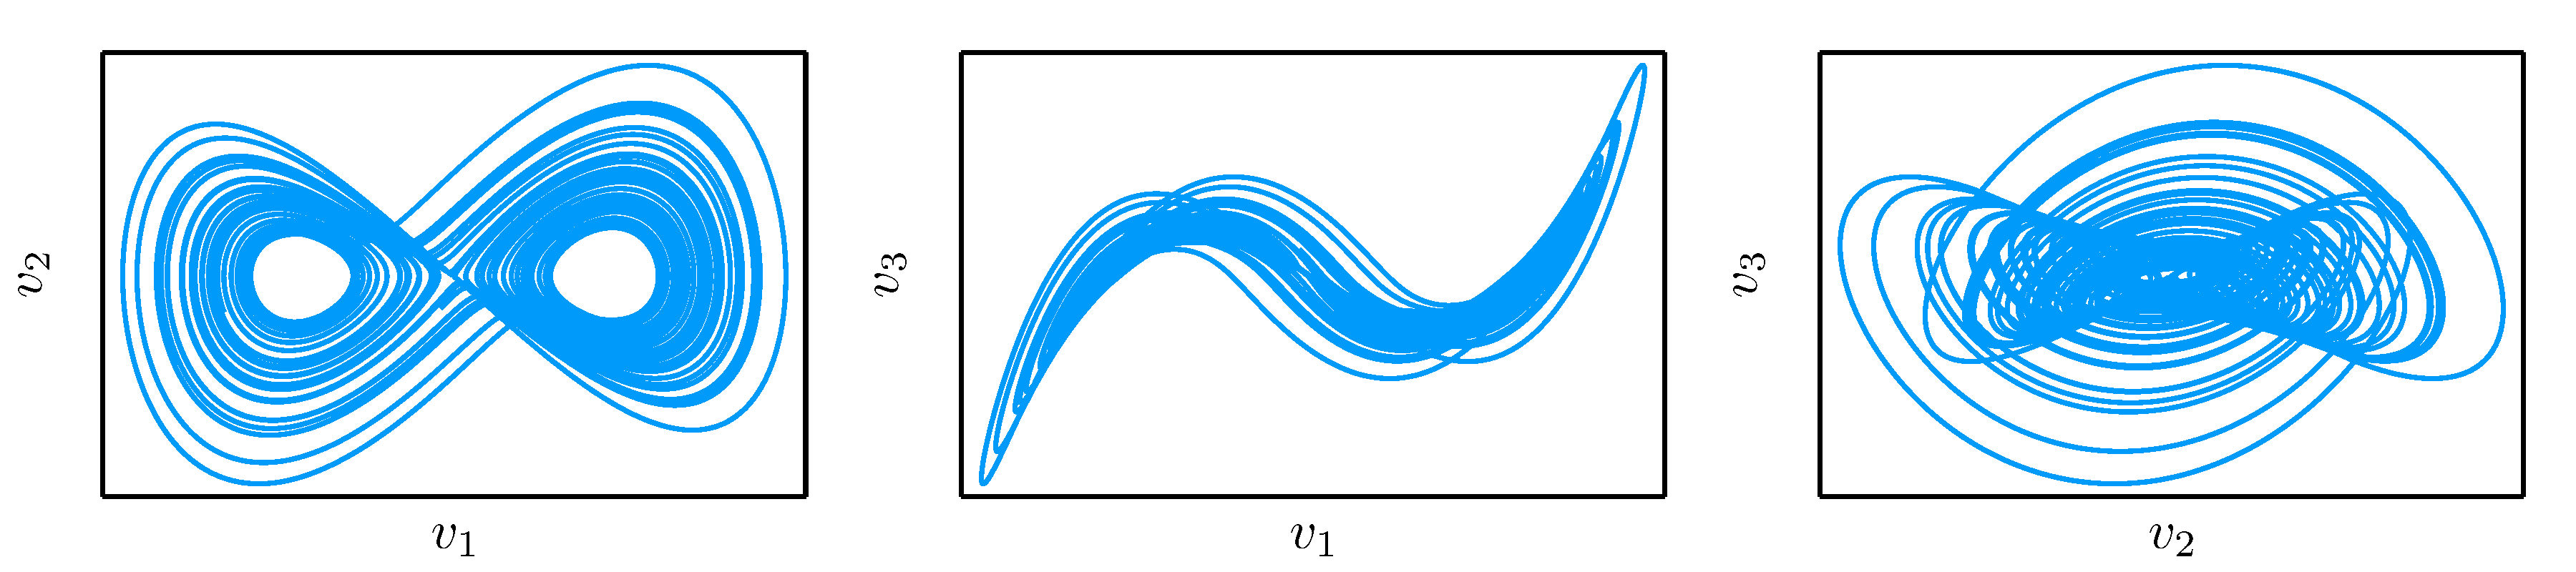
\includegraphics[width=\textwidth]{lorenz_broomhead_king_reconstruction}} \\
%       \subfigure[Poincaré section]{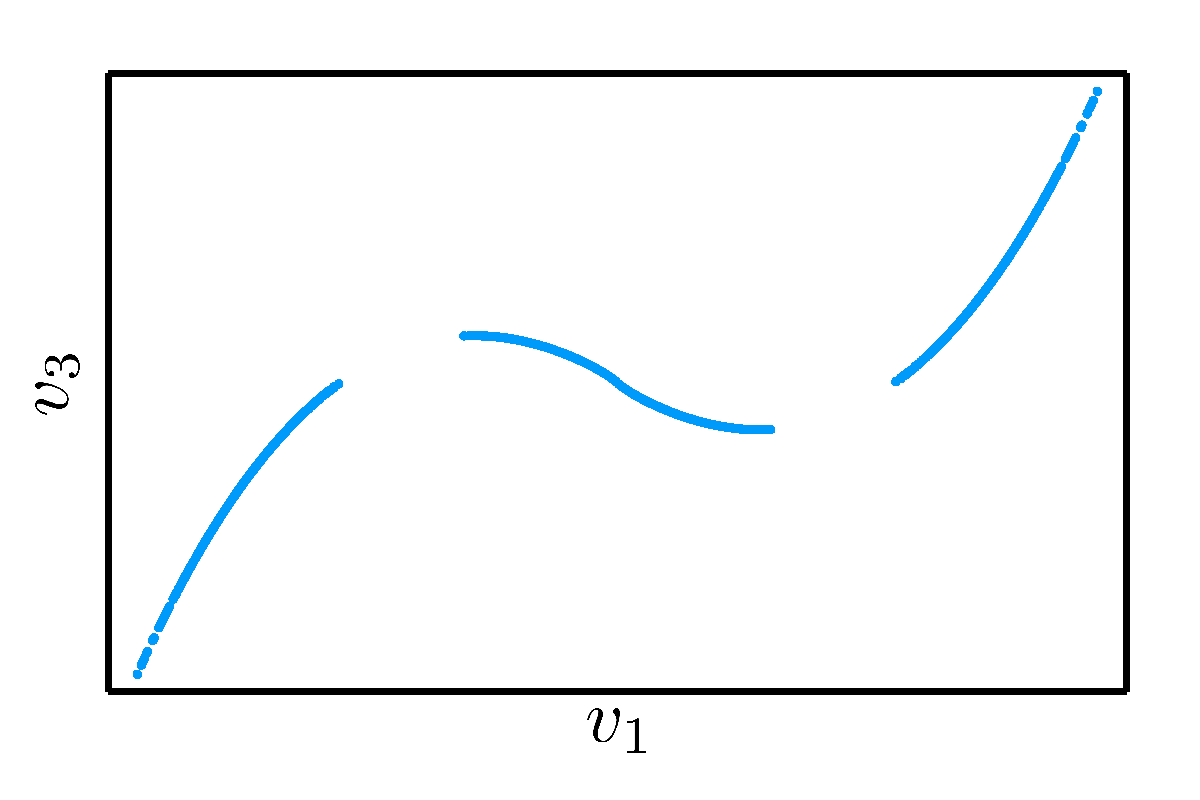
\includegraphics[width=.3333\textwidth]{lorenz_poincare_section}}
%     \end{figure}
%   \end{minipage}%
%   \hfill
%   \begin{minipage}{.48\textwidth}
%     \begin{figure}
%       \centering
%       \subfigure[Flow rate time series]{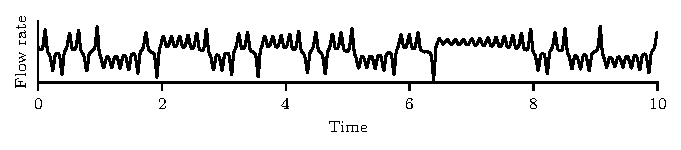
\includegraphics[width=\textwidth]{flow_rate_time_series}} \\
%       \subfigure[Attractor reconstruction]{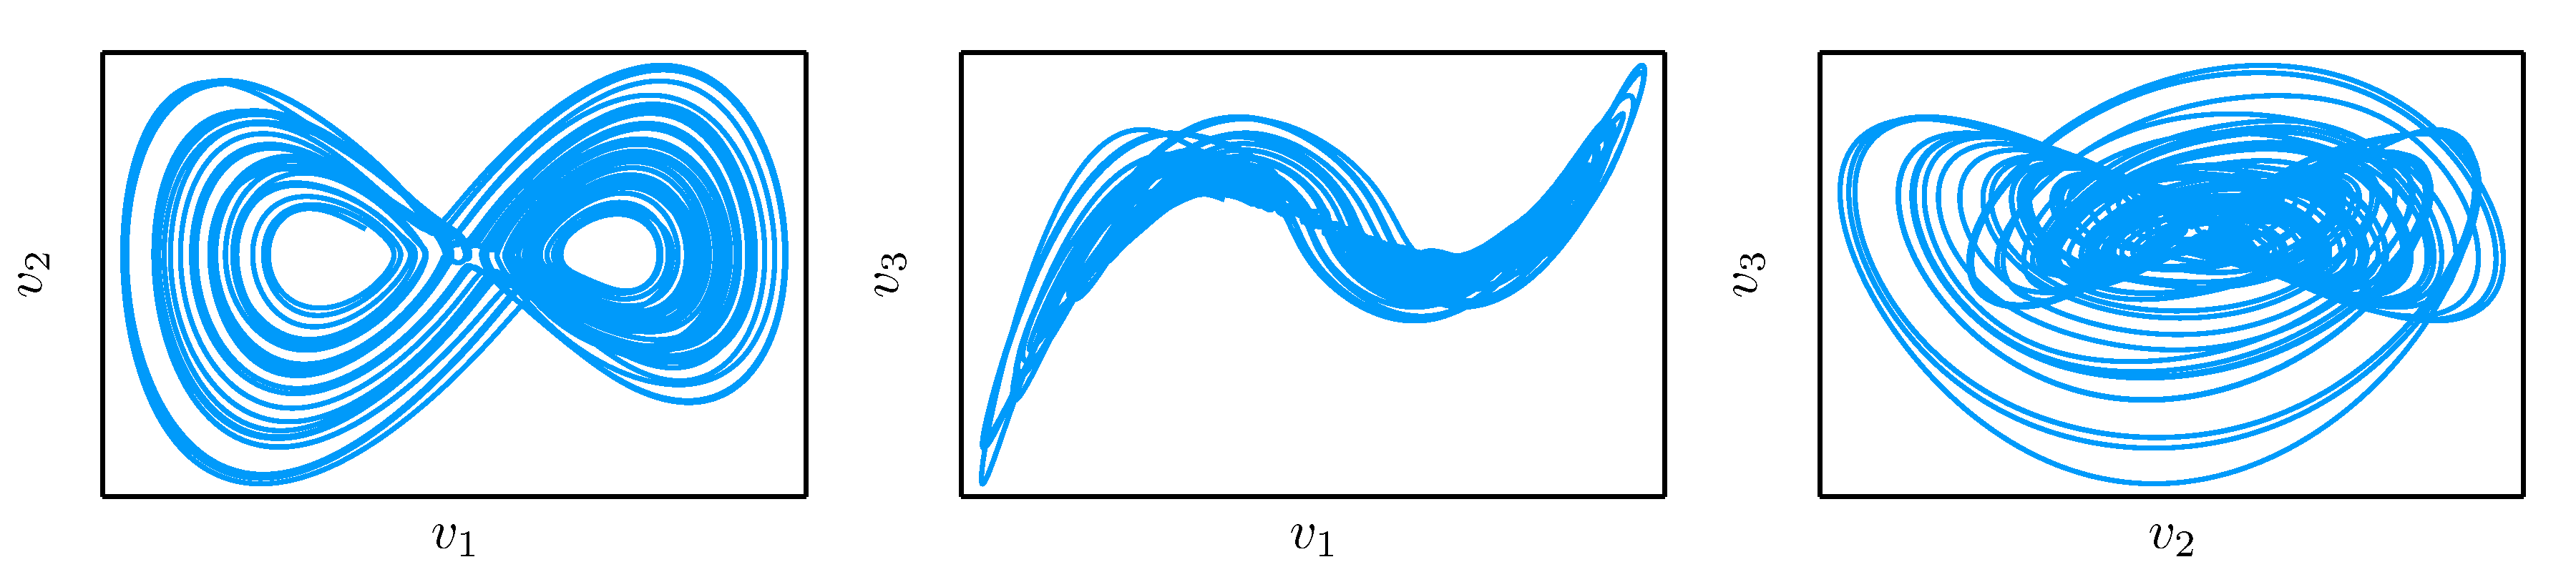
\includegraphics[width=\textwidth]{broomhead_king_reconstruction}} \\
%       \subfigure[Poincaré section]{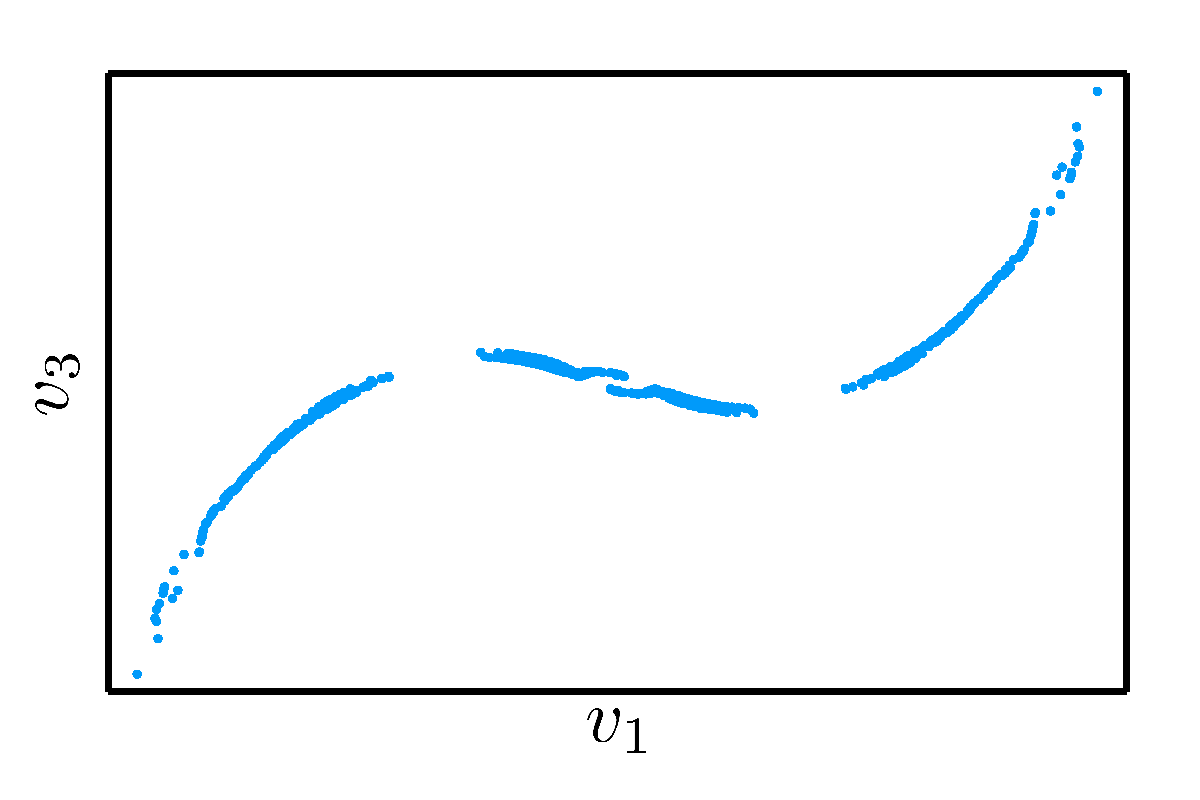
\includegraphics[width=.3333\textwidth]{flow_rate_poincare_section}}
%     \end{figure}
%   \end{minipage}
%
%   \vspace{1cm}
% \end{frame}


%%%%%
%%%%%
%%%%%
%%%%%
%%%%%

%%%%%%%%%%%%%%%%%%%%%%%%%%%%%%%%%%%%%%%%%%%%
%%%%%                                  %%%%%
%%%%%     DIMENSIONALITY REDUCTION     %%%%%
%%%%%                                  %%%%%     
%%%%%%%%%%%%%%%%%%%%%%%%%%%%%%%%%%%%%%%%%%%%     

\begin{frame}[t, c]{}{}
  \begin{minipage}{.48\textwidth}
    \centering
    {
      \Large\textbf{Part I}
    }
    
    \bigskip
    
    \rule{\textwidth}{0.001\textwidth}
    
    \bigskip
    
    {
      \large
      \textbf{Dimensionality reduction}
    }
    
    \medskip
    
    \begin{itemize}
    \item Problem formulation:
      \begin{itemize}
      \item[\(	\hookrightarrow \)] DMD as a Reduced Rank Regression
      \item[\( \hookrightarrow	\)] Linear autoencoder + linear dynamics
      \end{itemize}
      
      \medskip
      
    \item Practical usage:
      \begin{itemize}
      \item[\(	\hookrightarrow	\)] Extracting patterns from our flow
      \item[\(	\hookrightarrow \)] Low-dimensional embedding
      \end{itemize}
      
    \end{itemize}
    
  \end{minipage}%
  \hfill
  \begin{minipage}{.48\textwidth}
    \centering
    \movie[width=\textwidth, autostart, loop]{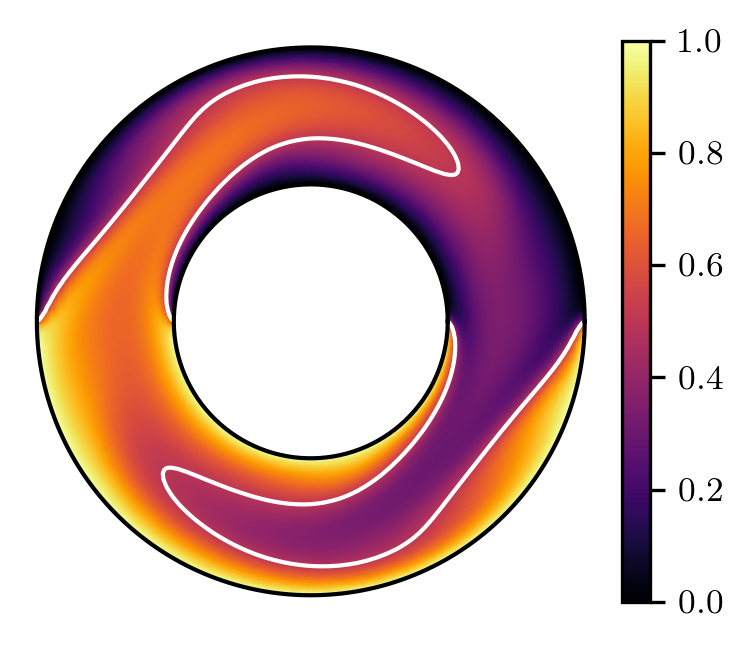
\includegraphics[width=\textwidth]{temperature_field_00000}}{imgs/temperature_evolution.mp4}
  \end{minipage}
\end{frame}

\begin{frame}[t, c]{Dynamic Mode Decomposition}{Problem formulation}
  \begin{minipage}{.68\textwidth}
    \begin{itemize}
    \item Given a discrete-time system \( \bm{x}_{k+1} = \bm{f}(\bm{x}_k) \), DMD aims to find a (low-rank) linear operator \( \bm{A} \) such that
      % 
      \[
        \begin{aligned}
          \minimize_{\bm{A}} & \sum_{k=1}^n \| \bm{f}(\bm{x}_k) - \bm{Ax}_k \|_2^2 \\
          \subjecto & \text{rank } \bm{A} = r.
        \end{aligned}
      \]
      
      \medskip
      
    \item This problem belongs to the class of \emph{Reduced-Rank Regression} problems.
    \end{itemize}
  \end{minipage}%
  \hfill
  \begin{minipage}{.28\textwidth}
    \centering
    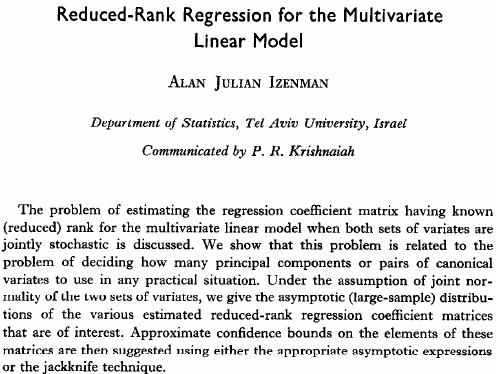
\includegraphics[width=\textwidth]{abstract_rrr}
  \end{minipage}
  
  \vspace{1cm}
\end{frame}

\begin{frame}[t, c]{Dynamic Mode Decomposition}{Matrix formulation and unconstrained solution}
  \begin{minipage}{.28\textwidth}
    \centering
    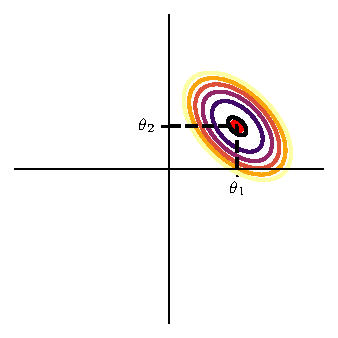
\includegraphics[width=\textwidth]{least_squares}
  \end{minipage}%
  \hfill
  \begin{minipage}{.68\textwidth}
    \begin{itemize}
    \item Problem can be recast in matrix form as
      % 
      \[
        \begin{aligned}
          \minimize_{\bm{A}} & \| \bm{Y} - \bm{AX} \|_F^2 \\
          \subjecto & \text{rank } \bm{A} = r,
        \end{aligned}
      \]
      % 
      where \( \bm{Y} = \bm{X}_{k+1} \) and \( \bm{X} = \bm{X}_k \).
      
      \medskip
      
    \item \underline{Unconstrained solution} is simply the least-squares solution
      % 
      \[
        \bm{A} = \bm{C}_{\bm{yx}} \bm{C}_{\bm{xx}}^{-1},
      \]
      % 
      with \( \bm{C}_{\bm{yx}} = \bm{YX}^H \) and \( \bm{C}_{\bm{xx}} = \bm{XX}^H \).
    \end{itemize}
  \end{minipage}
  
  \vspace{1cm}
\end{frame}

\begin{frame}[t, c]{Dynamic Mode Decomposition}{Rank-constrained solution}
  \begin{minipage}{.68\textwidth}
    \begin{itemize}
    \item Introducing the low-rank factorization \( \bm{A} = \bm{PQ}^H \), the minimization problem reads
      % 
      \[
        \begin{aligned}
          \minimize_{\bm{P}, \bm{Q}} & \| \bm{Y} - \bm{PQ}^H \bm{X} \|_F^2 \\
          \subjecto & \text{rank } \bm{P} = \text{rank } \bm{Q} = r \\
          & \bm{P}^H \bm{P} = \bm{I}.
        \end{aligned}
      \]
      
      \medskip
      
    \item \( \bm{P} \) is a basis for the column-span of \( \bm{A} \) while \( \bm{Q} \) is a basis for its row-span.
      These are in general different.
    \end{itemize}
  \end{minipage}%
  \hfill
  \begin{minipage}{.28\textwidth}
    \centering
    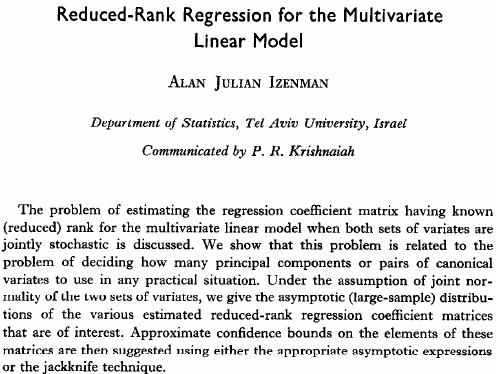
\includegraphics[width=\textwidth]{abstract_rrr}
  \end{minipage}
  
  \vspace{1cm}
\end{frame}

\begin{frame}[t, c]{Dynamic Mode Decomposition}{Rank-constrained solution}
  \begin{minipage}{.28\textwidth}
    \centering
    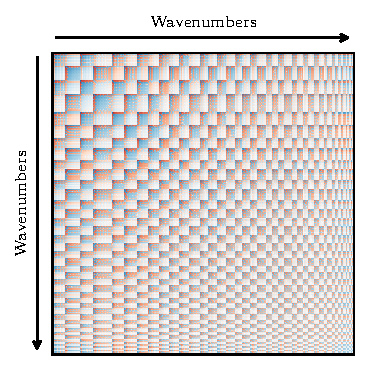
\includegraphics[width=\textwidth]{dmd_matrix}
  \end{minipage}%
  \hfill
  \begin{minipage}{.68\textwidth}
    \begin{itemize}
    \item Our minimization problem is equivalent to
      % 
      \[
        \begin{aligned}
          \maximize_{\bm{P}} & \text{Tr}\left( \bm{P}^H \bm{C}_{\bm{yx}} \bm{C}_{\bm{xx}}^{-1} \bm{C}_{\bm{xy}} \bm{P} \right) \\
          \subjecto & \text{rank } \bm{P} = r \\
          & \bm{P}^H \bm{P} = \bm{I}.
        \end{aligned}
      \]
      
      \medskip
      
    \item Optimal solution is given by the first \( r \) eigenvectors of the symmetric positive-definite matrix \( \bm{C}_{\bm{yx}} \bm{C}_{\bm{xx}}^{-1} \bm{C}_{\bm{xy}} \).
      
      \medskip
      
    \item \( \bm{Q} \) is solution to \( \bm{C}_{\bm{xx}} \bm{Q} =  \bm{C}_{\bm{xy}} \bm{P} \).
    \end{itemize}
  \end{minipage}
  
  \vspace{1cm}
\end{frame}

\begin{frame}[t, c]{Dynamic Mode Decomposition}{Dimensionality reduction and linear model}
  \begin{itemize}
  \item Once \( \bm{P} \) and \( \bm{Q} \) are found, \( \bm{A} \) may be factorized as \( \bm{A} = \boldsymbol{\Upphi} \boldsymbol{\Uplambda} \boldsymbol{\Uppsi}^H \).
  \end{itemize}
  
  \bigskip
  
  \centering
  
  \begin{tikzpicture}
    % \draw[help lines](0,0) grid (10,5);
    
    \node[fill=blue!20, minimum width=1cm, minimum height=3cm, rounded corners, draw=black, thick] (X) at (0, 2.5) {\( \bm{x}_k \)};
    
    \draw[fill=gray!10, thick] ([xshift=0.75cm]X.north east) -- ([xshift=2.75cm,yshift=0.5cm]X.east) -- ([xshift=2.75cm,yshift=-0.5cm]X.east) -- ([xshift=0.75cm]X.south east) -- cycle;
    \node at (2.25, 0.5) {\textsc{Encoder}};
    \node at (2.25, 2.5) {\( \boldsymbol{\Uppsi}^H \bm{x} = \bm{z} \)};
    
    \node[fill=gray!10, minimum width=2cm, minimum height=1.0cm, rounded corners, thick, draw=black] (Z) at (5cm, 2.5) {\( \boldsymbol{\Uplambda} \bm{z}_k = \bm{z}_{k+1}\)};
    \node at (5, 0.5) {\textsc{Dynamics}};
    
    \draw[fill=gray!10, thick] ([xshift=0.75cm]Z.north east) -- ([xshift=2.75cm,yshift=1cm]Z.north east) -- ([xshift=2.75cm,yshift=-1cm]Z.south east) -- ([xshift=0.75cm]Z.south east) -- cycle;
    \node at (7.75, 0.5) {\textsc{Decoder}};
    \node at (7.75, 2.5) {\( \boldsymbol{\Upphi} \bm{z} = \bm{x} \)};
    
    \node[fill=blue!20, minimum width=1cm, minimum height=3cm, rounded corners, draw=black, thick] (Xp) at (10, 2.5) {\( \bm{x}_{k+1} \)};
    
    \draw[arrow] (X.east) -- ([xshift=0.75cm]X.east);
    \draw[arrow] ([xshift=-0.75cm]Z.west) -- (Z.west);
    \draw[arrow] (Z.east) -- ([xshift=0.75cm]Z.east);
    \draw[arrow] ([xshift=-0.75cm]Xp.west) -- (Xp.west);
    
  \end{tikzpicture}
  
  \bigskip
  
  \begin{block}{}
    \textbf{Interpretation :} \( \ell_2 \)-optimal combination of linear autoencoder for dimensionality reduction and linear time-invariant model for the latent space (one-step ahead) dynamics.
  \end{block}
  
  \vspace{1cm}
\end{frame}

\begin{frame}[t, c]{Dynamic Mode Decomposition}{In practice}
  \begin{minipage}{.68\textwidth}
    \begin{itemize}
    \item Sampling period is heuristically chosen to be \( \nicefrac{\tau_0}{20} \).
      % \begin{itemize}
      % \item[\(	\hookrightarrow	\)] Large enough for the ``noise'' to decorrelate but small enough to correctly discretize the dominant frequencies.
      % \end{itemize}
      
      \bigskip
      
    \item DMD models are fitted separately for the velocity and temperature fields based on 20 000 snapshots.
      
      %\medskip
      
    %\item Provides a good embedding in the sense that the latent space dynamics are approximately linear.
      % \begin{itemize}
      % \item[\( \hookrightarrow	\)] Possible connection with normal form theory?
      % \end{itemize}
    \end{itemize}
  \end{minipage}%
  \hfill
  \begin{minipage}{.28\textwidth}
    \centering
    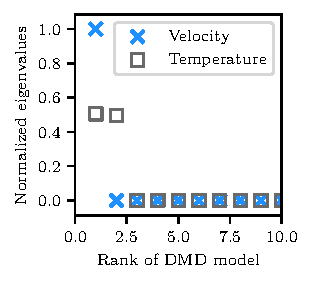
\includegraphics[width=\textwidth]{DMD_eigenspectrum}
    
    {\small
      Eigenspectrum of \( \bm{C}_{\bm{yx}} \bm{C}_{\bm{xx}}^{-1} \bm{C}_{\bm{xy}} \).
    }
  \end{minipage}
  
  \vspace{1cm}
\end{frame}

\begin{frame}[t, c]{Dynamic Mode Decomposition}{In practice}
  \begin{minipage}{.32\textwidth}
    \centering
    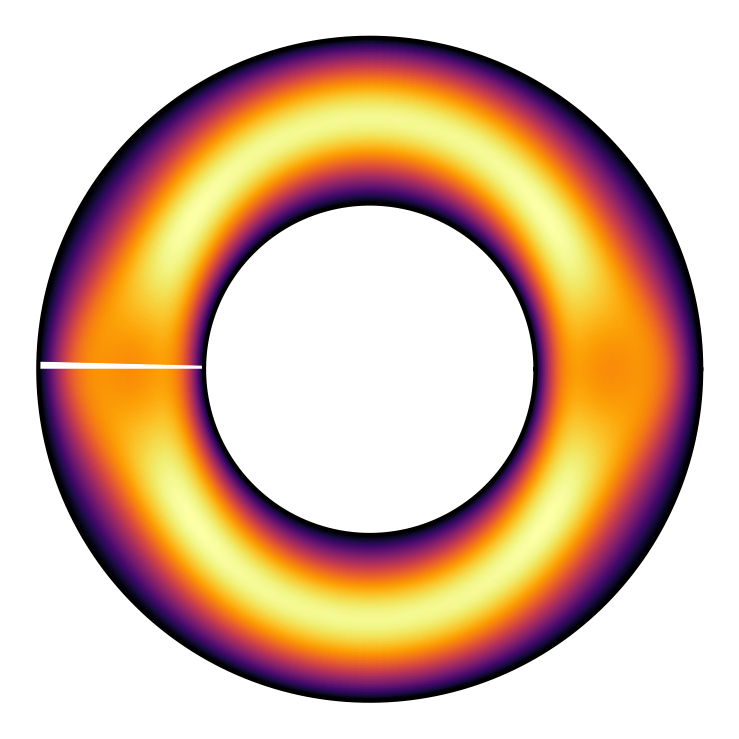
\includegraphics[width=\textwidth]{velocity_dmd_mode} \\
    
    {\small
      Leading DMD mode for the velocity.
    }
  \end{minipage}%
  \hfill
  \begin{minipage}{.32\textwidth}
    \centering
    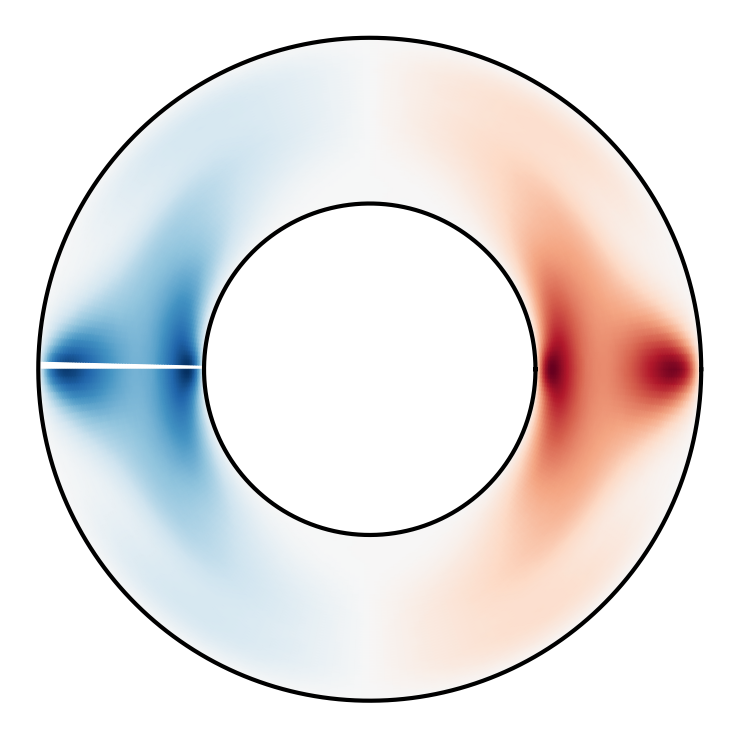
\includegraphics[width=\textwidth]{temperature_dmd_mode}
    
    {\small
      First DMD mode for the temperature.
    }
  \end{minipage}%
  \hfill
  \begin{minipage}{.32\textwidth}
    \centering
    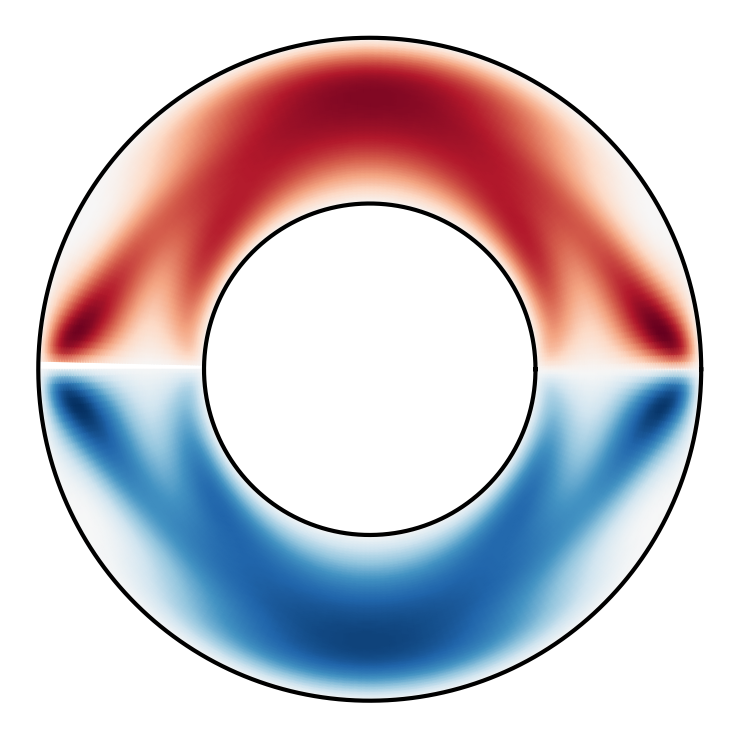
\includegraphics[width=\textwidth]{temperature_dmd_mode_bis}
    
    {
      \small
      Second DMD mode for the temperature.
    }
  \end{minipage}
  
  \vspace{1cm}
\end{frame}

\begin{frame}[t, c]{Dynamic Mode Decomposition}{In practice}
  \centering
  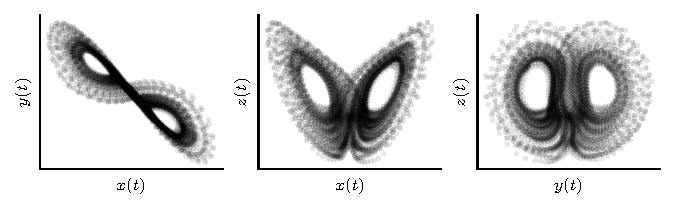
\includegraphics[width=.9\textwidth]{separate_low_dimensional_representation}
  
  \vspace{1cm}
\end{frame}


%%%%%
%%%%%
%%%%%
%%%%%
%%%%%

%%%%%%%%%%%%%%%%%%%%%%%%%%%%%%%%%%%%%%%%%
%%%%%                               %%%%%
%%%%%     STATISTICS OF CHAOTIC     %%%%%
%%%%%                               %%%%% 
%%%%%%%%%%%%%%%%%%%%%%%%%%%%%%%%%%%%%%%%% 

\begin{frame}[t, c]{}{}
  \begin{minipage}{.48\textwidth}
    \centering
    \begin{tikzpicture}
      \node[state] (s1) {\( \bm{s}_1 \)};
      \node[state, below right of=s1] (s2) {\( \bm{s}_2 \)};
      \node[state, below left of=s1] (s4) {\( \bm{s}_4 \)};
      \node[state, below left of=s2] (s3) {\( \bm{s}_3 \)};
      
      \draw (s1) edge[loop above] node {\(l_{11}\)} (s1);
      \draw (s1) edge[bend left] node {\(l_{21}\)}  (s2);
      
      \draw (s2) edge[loop right]  node {\(l_{22}\)} (s2);
      \draw (s2) edge[bend left]  node {\(l_{32}\)} (s3);
      
      \draw (s3) edge[bend left]  node {\(l_{43}\)} (s4);
      \draw (s3) edge[loop below]  node {\(l_{33}\)} (s3);
      
      \draw (s4) edge[bend left]  node {\(l_{14}\)} (s1);
      \draw (s4) edge[loop left]  node {\(l_{44}\)} (s4);
      
    \end{tikzpicture}
  \end{minipage}%
  \hfill
  \begin{minipage}{.48\textwidth}
    \centering
    {
      \Large\textbf{Part II}
    }
    
    \bigskip
    
    \rule{\textwidth}{0.001\textwidth}
    
    \bigskip
    
    {
      \large
      \textbf{Statistics of chaotic}
    }
    
    \medskip
    
    \begin{itemize}
    \item Problem formulation:
      \begin{itemize}
      \item[\(	\hookrightarrow \)] State space partition
      \item[\(	\hookrightarrow	\)] Cluster-based Reduced Order Modeling
      \end{itemize}
      
      \medskip
      
    \item Practical usage:
      \begin{itemize}
      \item[\(	\hookrightarrow	\)] Probabilistic model
      \item[\(	\hookrightarrow \)] Statistics of chaos
      \end{itemize}
      
    \end{itemize}
    
  \end{minipage}
\end{frame}

\begin{frame}[t, c]{Statistics of chaotic}{Overview}
  \begin{minipage}{.28\textwidth}
    \centering
    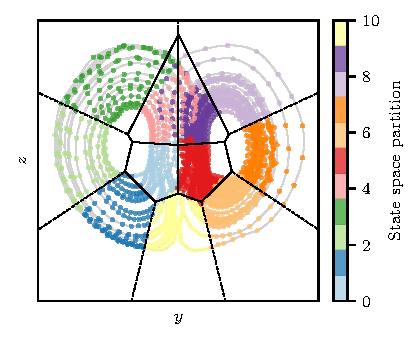
\includegraphics[width=\textwidth]{voronoi_diagram}
  \end{minipage}%
  \hfill
  \begin{minipage}{.68\textwidth}
    \begin{block}{}
      \centering
      \textbf{Cluster-based Reduced-Order Modeling}
    \end{block}
    
    \medskip
    
    \begin{itemize}
    \item \textbf{Aim:} Coarse-gain probabilistic model of the dynamics
      \begin{itemize}
      \item[\(	\hookrightarrow	\)] Linear model for the probability density function.
      \item[\(	\hookrightarrow	\)] Statistical properties of the system.
      \end{itemize}
      
      \medskip
      
    \item \textbf{How:} From continuous to symbolic dynamics.
      \begin{itemize}
      \item[\(	\hookrightarrow	\)] State-space partitionning using \underline{k-means}.
      \item[\(	\hookrightarrow	\)] Maximum likelihood estimation of the transition probability from cluster \( \bm{c}_i \) to cluster \( \bm{c}_j \).
      \end{itemize}
    \end{itemize}
  \end{minipage}
  
  \vspace{1cm}
\end{frame}

\begin{frame}[t, c]{Statistics of chaotic}{State-space partitionning}
  \begin{minipage}{.68\textwidth}
    \begin{itemize}
    \item Given a set of \( n \) observations \( (\bm{x}_1, \bm{x}_2, \cdots, \bm{x}_n) \), partition the data into \( k \) sets \( \bm{C} = \left\{ \bm{C}_1, \bm{C}_2, \cdots, \bm{C}_k \right\} \).
      
      \medskip
      
    \item To do so, \underline{k-means} aims to minimize the \emph{within-cluster sum of squares}
      % 
      \[
        \minimize_{\bm{C}} \sum_{i=1}^k \sum_{\bm{x} \in \bm{C}_i} \| \bm{x} - \bm{c}_i \|^2
      \]
      % 
      where \( \bm{c}_i \) is the centroid of the i\textsuperscript{th} cluster \( \bm{C}_i \).
    \end{itemize}
  \end{minipage}%
  \hfill
  \begin{minipage}{.28\textwidth}
    \centering
    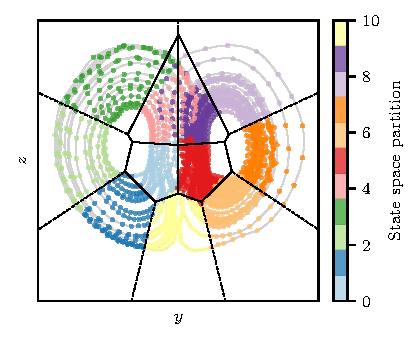
\includegraphics[width=\textwidth]{voronoi_diagram}
  \end{minipage}
  
  \vspace{1cm}
\end{frame}

\begin{frame}[t, c]{Statistics of chaotic}{State-space partitionning}
  \centering
  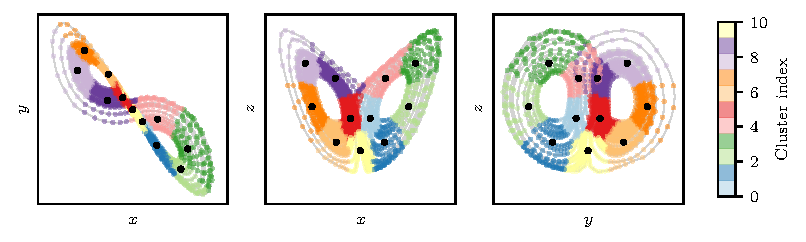
\includegraphics[width=\textwidth]{clustered_attractor}
  
  \vspace{1cm}
\end{frame}

\begin{frame}[t, c]{Statistics of chaotic}{Symbolic dynamics}
  \begin{minipage}{.48\textwidth}
    \centering
    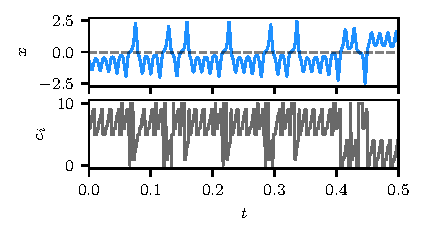
\includegraphics[width=\textwidth]{dns_crom_time_series}
  \end{minipage}%
  \hfill
  \begin{minipage}{.48\textwidth}
    \begin{itemize}
    \item Symbolic dynamics are obtained by looking at the evolution of the cluster index \( c(t) \).
      % \begin{itemize}
      % \item[\(	\hookrightarrow	\)] Dynamics on a finite set of \( k \) symbols.
      % \end{itemize}
      
      \medskip
      
    \item These dynamics can easily be modeled using a Markov chain.
      % \begin{itemize}
      % \item[\(	\hookrightarrow	\)] Transition matrix obtained from maximum likelihood estimation.
      % \end{itemize}
      
    \end{itemize}
  \end{minipage}
  
  \vspace{1cm}
\end{frame}

\begin{frame}[t, c]{Statistics of chaotic}{Markov chain model}
  \begin{minipage}{.68\textwidth}
    \begin{itemize}
    \item Using MLE, a Markov chain model
      % 
      \[
        \bm{p}_{k+1} = \bm{Lp}_k
      \]
      % 
      is identified where the i\textsuperscript{th} entry of \( \bm{p}_k \) describes the probability of being in cluster \( \bm{C}_i \) at time \( t = k \Delta T \).
      
      \medskip
      
    \item \( l_{ij} \) encodes the transition probability from cluster \( \bm{C}_j \) to cluster \( \bm{C}_i \) after one step.

    \end{itemize}
  \end{minipage}%
  \hfill
  \begin{minipage}{.28\textwidth}
    \centering
    \includegraphics[width=\textwidth]{CROM_transition_matrix} \\
    
    {\small
      Transition matrix \( \bm{L} \).
    }
  \end{minipage}
  
  \vspace{1cm}
\end{frame}

\begin{frame}[t, c]{Statistics of chaotic}{Markov chain model}
  \begin{minipage}{.68\textwidth}
    \begin{itemize}
      
    \item Existence of two ``mega-clusters'' corresponding to the clockwise and counter-clockwise rotation.
      
      \medskip
      
    \item When reaching the last cluster, the system to randomly switch from one side of the attractor to the other.
    \end{itemize}
  \end{minipage}%
  \hfill
  \begin{minipage}{.28\textwidth}
    \centering
    \includegraphics[width=\textwidth]{CROM_transition_matrix} \\
    
    {\small
      Transition matrix \( \bm{L} \).
    }
  \end{minipage}
  
  \vspace{1cm}
\end{frame}

\begin{frame}[t, c]{Statistics of chaotic}{Markov chain model}
  \centering
  \begin{tikzpicture}
    \node[state] (s2) at (36+0:2) {\( \bm{c}_2 \)};
    \node[state] (s3) at (36+72:2) {\( \bm{c}_3 \)};
    \node[state] (s4) at (36+144:2){\( \bm{c}_4 \)};
    \node[state] (s5) at (36+216:2) {\( \bm{c}_5 \)};
    \node[state] (s1) at (36+288:2) {\( \bm{c}_1 \)};
    
    \node[state, xshift=8cm] (s7) at (180-36:2) {\( \bm{c}_7 \)};
    \node[state, xshift=8cm] (s8) at (180-72-36:2) {\( \bm{c}_8 \)};
    \node[state, xshift=8cm] (s9) at (180-144-36:2) {\( \bm{c}_9 \)};
    \node[state, xshift=8cm] (s10) at (180-216-36:2) {\( \bm{c}_{10} \)};
    \node[state, xshift=8cm] (s6) at (180-288-36:2) {\( \bm{c}_6 \)};
    
    \node[state, xshift=4cm] (s11) at (0, 0) {\( \bm{c}_{11} \)};
    
    \draw (s1) edge[bend right, red] node {}  (s2);
    \draw (s1) edge[bend right, red!50] node {} (s11);
    \draw (s1) edge[bend right, red!25] node {} (s6);
    
    \draw (s2) edge[bend right, red] node {} (s3);
    
    \draw (s3) edge[bend right, red] node {} (s4);
    
    \draw (s4) edge[bend right, red] node {} (s5);
    
    \draw (s5) edge[bend right, red] node {} (s1);
    
    
    \draw (s6) edge[bend left, red] node {} (s7);
    \draw (s6) edge[bend left, red!50] node {} (s11);
    \draw (s6) edge[bend left, red!25] node {} (s1);
    
    \draw (s7) edge[bend left, red] node {} (s8);
    
    \draw (s8) edge[bend left, red] node {} (s9);
    
    \draw (s9) edge[bend left, red] node {} (s10);
    
    \draw (s10) edge[bend left, red] node {} (s6);
    
    \draw (s11) edge[bend right, red] node {} (s2);
    \draw (s11) edge[bend left, red] node {} (s7);
    
    \node at (0, 0) {\textsc{Clockwise}};
    \node at (8, 0) {\textsc{Anticlockwise}};
    
  \end{tikzpicture}
  
  \vspace{1cm}
\end{frame}

\begin{frame}[t, c]{Statistics of chaotic}{Statistical analysis}
  \begin{minipage}{.68\textwidth}
    \begin{itemize}
    \item Eigenspectrum of \( \bm{L} \) encodes the diffusion of the probability density function.
      
      \bigskip
      
    \item Eigenvector \( \bm{p}^{\infty} \) associated to \( \lambda_1 = 1 \) characterizes the invariant measure (i.e. the long-time/ensemble average distribution of \( \bm{p} \)).
    \end{itemize}
    
    \bigskip
    
    \centering
    \includegraphics[width=.8\textwidth]{probability_distribution}
  \end{minipage}%
  \hfill
  \begin{minipage}{.28\textwidth}
    \centering
    \includegraphics[height=.666\textheight]{CROM_eigenspectrum}
  \end{minipage}
  
  \vspace{1cm}
\end{frame}

\begin{frame}[t, c]{Statistics of chaotic}{Statistical analysis}
  \begin{minipage}{.68\textwidth}
    \begin{itemize}
    \item How fast the p.d.f.\ diffuses is related to the ratio \( \nicefrac{\vert \lambda_2 \vert}{\vert \lambda_1 \vert} \).
      \begin{itemize}
      \item[\( \hookrightarrow	\)] The larger it is, the faster the p.d.f.\ converges to its invariant measure.
      \end{itemize}
      
      \medskip
      
    \item \( \vert \lambda_2 \vert^k \) provides an estimate of how far in time we can predict.
      \begin{itemize}
      \item[\( \hookrightarrow	\)] Our prediction horizon is only one characteristic time-scale.
      \end{itemize}
    \end{itemize}
    
    \medskip
    
    \centering
    \includegraphics[width=.8\textwidth]{convergence_crom}
  \end{minipage}%
  \hfill
  \begin{minipage}{.28\textwidth}
    \centering
    \includegraphics[width=\textwidth]{voronoi_diagram}
  \end{minipage}
  
  \vspace{1cm}
\end{frame}


%%%%%
%%%%%
%%%%%
%%%%%
%%%%%

%%%%%%%%%%%%%%%%%%%%%%%%%%%%%%%%%%%%%%%%%
%%%%%                               %%%%%
%%%%%     SYSTEM IDENTIFICATION     %%%%%
%%%%%                               %%%%%
%%%%%%%%%%%%%%%%%%%%%%%%%%%%%%%%%%%%%%%%%

\begin{frame}[t, c]{}{}
  \begin{minipage}{.48\textwidth}
    \centering
    % \includegraphics[width=\textwidth]{cover}
    \movie[autostart, loop, width=\textwidth]{
      \includegraphics[width=\textwidth]{imgs/lorenz.png}}{imgs/lorenz.wmv}
  \end{minipage}%
  \hfill
  \begin{minipage}{.48\textwidth}
    \centering
    {
      \Large\textbf{Part III}
    }
    
    \bigskip
    
    \rule{\textwidth}{0.001\textwidth}
    
    \bigskip
    
    {
      \large
      \textbf{Sparse Identification of Nonlinear Dynamics}
    }
    
    \medskip
    
    \begin{itemize}
    \item Problem formulation:
      % 
      \begin{itemize}
      \item[\(	\hookrightarrow	\)] Physical constraints
      \item[\(	\hookrightarrow	\)] Optimization problem
      \item[\(	\hookrightarrow	\)] Greedy algorithms and convex relaxations
      \end{itemize}
      
      \medskip
      
    \item Application to the chaotic thermosyphon:
      \begin{itemize}
      \item[\(	\hookrightarrow	\)] A Lorenz-like system
      \item[\(	\hookrightarrow	\)] Cross-validations
      \end{itemize}
      
    \end{itemize}
    
  \end{minipage}
\end{frame}

\begin{frame}[t, c]{Identifying a dynamical system}{Overview}
  \begin{minipage}{.48\textwidth}
    \begin{block}{}
      \centering
      \textbf{Sparse Identification of Nonlinear Dynamics}
    \end{block}
    
    \medskip
    
    \begin{itemize}
    \item \textbf{Aim:} Identify a low-order nonlinear dynamical system
      \begin{itemize}
      \item[\(	\hookrightarrow	\)] Inherently interpretable set of ODE.
      \item[\(	\hookrightarrow	\)] Fast evaluation for forecasting.
      \end{itemize}
      
      \medskip
      
    \item \textbf{How:} Sparse least-squares regression
      \begin{itemize}
      \item[\(	\hookrightarrow	\)] Constraints for physical consistency.
      \item[\(	\hookrightarrow	\)] Greedy algorithms/convex relaxations.
      \end{itemize}
    \end{itemize}
  \end{minipage}%
  \hfill
  \begin{minipage}{.48\textwidth}
    \centering
    \includegraphics[width=\textwidth]{physics_machine_learning}
  \end{minipage}
  
  \vspace{1cm}
\end{frame}

\begin{frame}[t, c]{Sparse Identification of Nonlinear Dynamics}{Overview}
  \begin{minipage}{.48\textwidth}
    \begin{itemize}
    \item Brunton \emph{et al.}, \emph{Proc. Natl. Acad. Sci. U.S.A.}, 2015.
      
      \medskip
      
    \item Relies on a dictionnary of pre-defined functions and sparsity-promoting regression.
      
      \medskip
      
    \item Quite promissing and versatile framework.
    \end{itemize}
  \end{minipage}%
  \hfill
  \begin{minipage}{.48\textwidth}
    \centering
    \includegraphics[width=\textwidth]{sindy_paper}
  \end{minipage}
  
  \vspace{1cm}
\end{frame}

\begin{frame}[t, c]{Sparse Identification of Nonlinear Dynamics}{A combinatorial problem}
  \begin{minipage}{.48\textwidth}
    \centering
    \includegraphics[width=\textwidth]{sparse_identification}
  \end{minipage}%
  \hfill
  \begin{minipage}{.48\textwidth}
    \begin{itemize}
    \item Given \(	\boldsymbol{\Uptheta}(\bm{x})	\), one aims to solve
      % 
      \[
        \begin{aligned}
          \minimize_{\boldsymbol{\upxi}} & \text{card }(\boldsymbol{\upxi}) \\
          \subjecto & \| \boldsymbol{\Uptheta}(\bm{x}) \boldsymbol{\upxi} - \dot{\bm{x}} \|_2^2 \leq \sigma.
        \end{aligned}
      \]
      
    \item Rapidly intractable combinatorial problem.
      
      \medskip
      
    \item Convex relaxation and/or greedy algorithms needed.
    \end{itemize}
  \end{minipage}
  
  \vspace{1cm}
\end{frame}

\begin{frame}[t, c]{Sparse Identification of Nonlinear Dynamics}{Problem formulation: general form}
  \begin{itemize}
  \item Navier-Stokes are nonlinear PDEs with quadratic nonlinearities so the dictionnary is chosen as
    % 
    \[
      \boldsymbol{\Uptheta}(\bm{x}) = \begin{bmatrix} 1 & x & y & z & x^2 & xy & xz & y^2 & yz & z^2 \end{bmatrix}.
    \]
    
    \medskip
    
  \item The yet-unknown model takes the following general form
    % 
    \[
      \begin{aligned}
        \dot{x} & = a_0 + a_1 x + a_2 y + a_3 z + a_4 x^2 + a_5 xy + a_6 xz + a_7 y^2 + a_8 yz + a_9 z^2 \\
        \dot{y} & = b_0 + b_1 x + b_2 y + b_3 z + b_4 x^2 + b_5 xy + b_6 xz + b_7 y^2 + b_8 yz + b_9 z^2 \\
        \dot{z} & = c_0 + c_1 x + c_2 y + c_3 z + c_4 x^2 + c_5 xy + c_6 xz + c_7 y^2 + c_8 yz + c_9 z^2
      \end{aligned}
    \]
    
    \medskip
    
  \item Up to 30 coefficients need to be identified using our training data.
  \end{itemize}
  
  \vspace{1cm}
\end{frame}

\begin{frame}[t, c]{Sparse Identification of Nonlinear Dynamics}{Problem formulation: equivariant system}
  \begin{minipage}{.68\textwidth}
    \begin{itemize}
    \item System is equivariant w.r.t.\ to the transformation \( (x, y, z) \mapsto (-x, -y, z) \).
      We thus have
      % 
      \[
        \gamma \cdot \dot{\bm{x}} = \bm{f}\left( \gamma \cdot \bm{x} \right)
      \]
      % 
      with \( \gamma \) the matrix representation of the flip operator.
      
      \smallskip
      
    \item The yet-unknown model reduces to
      % 
      \[
        \begin{aligned}
          \dot{x} & = a_0 x + a_1 y + a_2 xz + a_3 yz \\
          \dot{y} & = b_0 x + b_1 y + b_2 xz + b_3 yz \\
          \dot{z} & = c_0 + c_1 z + c_2 x^2 + c_3 xy + c_4 y^2 + c_5 z^2
        \end{aligned}
      \]
      
      \smallskip
      
    \item Only 14 terms need to be actually identified.
      
    \end{itemize}
  \end{minipage}%
  \hfill
  \begin{minipage}{.28\textwidth}
    \centering
    \includegraphics[width=\textwidth]{flip_symmetry}
  \end{minipage}
  
  \vspace{1cm}
\end{frame}

\begin{frame}[t, c]{Sparse Identification of Nonlinear Dynamics}{Problem formulation: dissipative system}
  \begin{minipage}{.28\textwidth}
    \centering
    \movie[width=\textwidth]{\includegraphics[width=\textwidth]{dissipative_system}}{imgs/dissipative_system.mp4}
  \end{minipage}%
  \hfill
  \begin{minipage}{.68\textwidth}
    \begin{itemize}
    \item The system \( \dot{\bm{x}} = \bm{f}(\bm{x}) \) is \underline{dissipative}, thus
      % 
      \[
        \nabla \cdot \bm{f}(\bm{x}) < 0 \quad \forall \bm{x}.
      \]
      
      \medskip
      
    \item It yields to the following constraints
      % 
      \[
        \begin{aligned}
          a_0 + b_1 + c_1 & < 0, \\
          a_2 + b_3 + 2c_5 & = 0.
        \end{aligned}
      \]
      
      \medskip
      
    \item All three equations are coupled by these constraints and need to be identified jointly.
    \end{itemize}
  \end{minipage}
  
  \vspace{1cm}
\end{frame}

\begin{frame}[t, c]{Sparse Identification of Nonlinear Dynamics}{Problem formulation: energy-preserving quadratic nonlinearities}
  \begin{minipage}{.58\textwidth}
    \begin{itemize}
    \item Quadratic nonlinearities in Navier-Stokes are energy-preserving.
      
      \medskip
      
    \item For our system, energy equation would read
      % 
      \[
        \dot{E} = c_0 z + a_0 x^2 + b_1 y^2 + c_1 z^2 + (a_1 + b_0) xy.
      \]
      
    \item The following constraints need to be satistifed
      % 
      \[
        \begin{aligned}
          & b_3 + c_4 = 0, \quad a_2 + c_2 = 0 \\
          & a_3 + b_2 + c_3 = 0.
        \end{aligned}
      \]
    \end{itemize}
  \end{minipage}%
  \hfill
  \begin{minipage}{.38\textwidth}
    \begin{equation}
      \begin{aligned}
        \textrm{State equation : } & \dot{\bm{x}} = \bm{b} + \bm{Ax} + \mathcal{Q}(\bm{x}) \\
        \textrm{Energy : } & E = \frac{1}{2} \bm{x}^T \bm{x} \\
        \textrm{Energy equation : } & \dot{E} = \bm{x}^T \left( \bm{b} + \bm{Ax} \right)
      \end{aligned}
      \notag
    \end{equation}
  \end{minipage}
  
  \vspace{1cm}
\end{frame}

\begin{frame}[t, c]{Sparse Identification of Nonlinear Dynamics}{Final problem}
  \begin{minipage}{.58\textwidth}
    \begin{overprint}
      \onslide<1>
      Our optimization problem finally takes the following form
      % 
      \[
        \begin{aligned}
          \minimize_{\boldsymbol{\upxi}} & \text{card}(\boldsymbol{\upxi}) \\
          \subjecto & \| \boldsymbol{\Uptheta}(\bm{x}) \boldsymbol{\upxi} - \dot{\bm{x}} \|_2^2 < \sigma \\
          & \bm{C} \boldsymbol{\upxi} = 0 \\
          & \bm{D} \boldsymbol{\upxi} < 0.
        \end{aligned}
      \]
      % 
      with \( \boldsymbol{\upxi} = \begin{bmatrix} \boldsymbol{\upxi}_x & \boldsymbol{\upxi}_y & \boldsymbol{\upxi}_z \end{bmatrix}^T \) the vector of unknown coefficients.
      
      \onslide<2>
      In practice, this combinatorial problem is approximated by a convex relaxation, e.g.
      % 
      \[
        \begin{aligned}
          \minimize_{\boldsymbol{\upxi}} & \| \boldsymbol{\Uptheta}(\bm{x}) \boldsymbol{\upxi} - \dot{\bm{x}} \|_2^2 + \lambda R(\boldsymbol{\upxi}) \\
          \subjecto & \bm{C} \boldsymbol{\upxi} = 0 \\
          & \bm{D} \boldsymbol{\upxi} < 0,
        \end{aligned}
      \]
      % 
      with \( R(\bm{x}) \) some sparsity promoting heuristic.
      Here, we chose \( R(\bm{x}) = \| \boldsymbol{\upxi} \|_2^2 \) (i.e.\ Thikonov regularization).
    \end{overprint}
  \end{minipage}%
  \hfill
  \begin{minipage}{.38\textwidth}
    \centering
    \includegraphics[width=\textwidth]{sparse_identification}
  \end{minipage}
  
  \vspace{1cm}
\end{frame}

\begin{frame}[t, c]{Sparse Identification of Nonlinear Dynamics}{Identifying the model}
  \begin{minipage}{.68\textwidth}
    \begin{itemize}
    \item Our dataset spans \( 500 \tau \) time-units.
      A sequence of \( 400 \tau \) is used for training while the remaining \( 100 \tau \) are used for testing.
      
      \medskip
      
    \item The optimization problem is implemented using the python bindings of \texttt{cvxopt}.
      
      \medskip
      
    \item Model selection is based on the ability of the identified system to reproduce the second-order statistics of the true system.
    \end{itemize}
  \end{minipage}%
  \hfill
  \begin{minipage}{.28\textwidth}
    \centering
    \includegraphics[width=\textwidth]{latent_space}
  \end{minipage}
  
  \vspace{1cm}
\end{frame}

\begin{frame}[t, c]{Sparse Identification of Nonlinear Dynamics}{Identified systems and model selection}
  \centering
  \includegraphics[width=.9\textwidth]{KL_divergence_model_selection}
  
  {\small
    \[
      \textrm{KL}(\bm{A} \vert \bm{B}) = \frac{1}{2} \left( \textrm{Tr}(\bm{B}^{-1}\bm{A}) - n + \ln \frac{\vert \bm{B} \vert}{\vert \bm{A} \vert} \right)
    \]
  }
  
  \vspace{1cm}
\end{frame}

\begin{frame}[t, c]{Sparse Identification of Nonlinear Dynamics}{Selected model}
  \begin{minipage}{.68\textwidth}
    
    \begin{block}{\centering \textbf{Selected model}}
      \[
        \begin{aligned}
          \dot{x} & = -76.08 x + 88.39 y \\
          \dot{y} & = 20.76 x - 4.19 y - 41.49 xz \\
          \dot{z} & = -43.67 - 17.31 z + 41.49 xy.
        \end{aligned}
      \]
    \end{block}
    
    \medskip
    
    \begin{itemize}
    \item \underline{Lorenz-like} system satisfying all of the physical constraints by design.
      
      \medskip
      
    \item Every single term can be intepreted and associated to a particular physical mechanism.
    \end{itemize}
  \end{minipage}%
  \hfill
  \begin{minipage}{.28\textwidth}
    \centering
    \includegraphics[width=\textwidth]{attractor_comparison}
  \end{minipage}
  
  \vspace{1cm}
\end{frame}

\begin{frame}[t, c]{Sparse Identification of Nonlinear Dynamics}{Selected model}
  \centering
  \includegraphics[width=.9\textwidth]{attractor_comparison_bis}
\end{frame}


% \begin{frame}[t, c]{Sparse Identification of Nonlinear Dynamics}{Physical mechanisms at play}
%   \centering
  
%   \begin{overprint}
%     \onslide<1>
%     \centering
%     \includegraphics[height=.7\textheight]{high_level_description}
    
%     \onslide<2>
%     \centering
%     \includegraphics[height=.7\textheight]{high_level_description_x}
    
%     \onslide<3>
%     \centering
%     \includegraphics[height=.7\textheight]{high_level_description_y}
    
%     \onslide<4>
%     \centering
%     \includegraphics[height=.7\textheight]{high_level_description_z}
    
%   \end{overprint}
  
%   \vspace{1cm}
% \end{frame}


\begin{frame}[t, c]{Sparse Identification of Nonlinear Dynamics}{Comparing the statistical properties}
  \begin{minipage}{.48\textwidth}
    \centering
    \includegraphics[width=.95\textwidth]{autocorrelation_function_comparison}

  \end{minipage}%
  \hfill
  \begin{minipage}{.48\textwidth}
    \includegraphics[width=.95\textwidth]{time_scale_distribution_comparison}
  \end{minipage}

  \bigskip
  
  \centering
  The model accurately captures the dynamical properties of the switches.
  
  \vspace{1cm}
\end{frame}

\begin{frame}[t, c]{Sparse Identification of Nonlinear Dynamics}{Comparing the statistical properties}

  \begin{center}
    \includegraphics[width=.8\textwidth]{probability_density_functions}
  \end{center}

  \medskip

  Overall agreements regarding the probability density functions albeit there is a small (yet unexplained) mismatch in the center.
  \vspace{1cm}
\end{frame}

% \begin{frame}[t, c]{Sparse Identification of Nonlinear Dynamics}{Quantitative comparison with the true system}
%   \begin{minipage}{.28\textwidth}
%     \begin{overprint}
%       \onslide<1>
%       \centering
%       \includegraphics[width=\textwidth]{pdf_comparison_x}
      
%       \onslide<2>
%       \centering
%       \includegraphics[width=\textwidth]{pdf_comparison_y}
      
%       \onslide<3>
%       \centering
%       \includegraphics[width=\textwidth]{pdf_comparison_z}
%     \end{overprint}
%   \end{minipage}%
%   \hfill
%   \begin{minipage}{.68\textwidth}
%     \begin{itemize}
%     \item Time-scale distribution is reasonnably well-captured.
%       \begin{itemize}
%       \item[\( \hookrightarrow	\)] Mismatch is \( \mathcal{O}(\Delta t) \).
%       \end{itemize}
      
%       \medskip
      
%     \item Marginal and joint p.d.f.\ are predicted correctly by the model except in the vicinity of \( x = y = 0 \).
%       \begin{itemize}
%       \item[\(	\hookrightarrow	\)] Further physical analyses needed.
%       \end{itemize}
%     \end{itemize}
    
%     \medskip
    
%     \centering
%     \includegraphics[width=.8\textwidth]{time_scale_distribution_comparison}
%   \end{minipage}
  
%   \vspace{1cm}
% \end{frame}

\begin{frame}[t, c]{Sparse Identification of Nonlinear Dynamics}{Forecasting abilities}
  \begin{minipage}{.48\textwidth}
    \begin{itemize}
    \item The identified model can easily be used for forecasting.
      
      \medskip
      
    \item Some specific regions of phase space are prone to large forecasting errors.
      
      \medskip
      
    \item Forecasts are statistically accurate on the characteristic time-scale \( \tau \).
    \end{itemize}
  \end{minipage}%
  \hfill
  \begin{minipage}{.48\textwidth}
    \begin{overprint}
      \onslide<1>
      \centering
      \includegraphics[width=\textwidth]{bad_forecast}
      
      \onslide<2>
      \centering
      \includegraphics[width=\textwidth]{good_forecast}
      
    \end{overprint}
  \end{minipage}
  
  \vspace{1cm}
\end{frame}

\begin{frame}[t, c]{Sparse Identification of Nonlinear Dynamics}{Eyeball-norm comparison}
  \begin{minipage}{.48\textwidth}
    \centering
    \begin{block}{}
      \centering
      \textbf{Direct numerical simulation}
    \end{block}
    \centering
  
    \movie[width=\textwidth, autostart, loop]{\centering \includegraphics[width=.8\textwidth]{ground_truth}}{imgs/ground_truth.mp4}
  \end{minipage}%
  \hfill
  \begin{minipage}{.48\textwidth}
    \centering
    \begin{block}{}
      \centering
      \textbf{Reduced-order model}
    \end{block}
    \centering
    \movie[width=\textwidth, autostart, loop]{\centering \includegraphics[width=.8\textwidth]{rom_predict}}{imgs/rom_predict.mp4}
  \end{minipage}
  \vspace{1cm}
\end{frame}

%%%%%
%%%%%
%%%%%
%%%%%
%%%%%

\begin{frame}[t, c]{}{}
  \begin{minipage}{.48\textwidth}
    \centering
    \includegraphics[width=.7\textwidth]{42}
  \end{minipage}%
  \hfill
  \begin{minipage}{.48\textwidth}
    \centering
    {
      \Large\textbf{Part IV}
    }
    
    \bigskip
    
    \rule{\textwidth}{0.001\textwidth}
    
    \bigskip
    
    {
      \large
      \textbf{Random thoughts on life, the universe and everything}
    }
    % \begin{itemize}
    % \item Summary
    % 
    % \medskip
    % 
    % \item Random thoughts and open problems.
    % \end{itemize}
    
  \end{minipage}
\end{frame}

\begin{frame}[t, c]{Random thoughts on life, the universe and everything}{Dimensionality reduction}
  \begin{minipage}{.68\textwidth}
    \begin{itemize}
    \item Dimensionality reduction as a preprocessing step to model the dynamics of physical systems has two competing objectives
      % 
      \begin{enumerate}
      \item Project the data in a low-dimensional latent space.
      \item The resulting coordinate system needs to be well-suited for modeling dynamics.
      \end{enumerate}
      
      \medskip
      
    \item While goal n\textsuperscript{o}1 can easily be formalized mathematically, goal n\textsuperscript{o}2 is more abstract.
    \end{itemize}
  \end{minipage}%
  \hfill
  \begin{minipage}{.28\textwidth}
    \centering
    \includegraphics[width=\textwidth]{latent_space}
  \end{minipage}
  
  \vspace{1cm}
\end{frame}

\begin{frame}[t, c]{Random thought on life, the universe and everything}{Dimensionality reduction}
  \begin{minipage}{.68\textwidth}
    \begin{itemize}
    \item Given full-state data, personnal experience suggests that DMD-like techniques are well-suited.
      \begin{itemize}
      \item[\(	\hookrightarrow	\)] Relies on highly-efficient numerical linear algebra techniques.
      \item[\(	\hookrightarrow	\)] Inherently interpretable low-dimensional phase space.
      \end{itemize}
      
      \medskip
      
    \item From a dynamical system point of view, DMD has been related to the Koopman operator.
      \begin{itemize}
      \item[\(	\hookrightarrow	\)] Provides a coordinate system where the dynamics are approximately linear.
      \end{itemize}
    \end{itemize}
  \end{minipage}%
  \hfill
  \begin{minipage}{.28\textwidth}
    \centering
    \includegraphics[width=\textwidth]{latent_space}
  \end{minipage}
  
  \vspace{1cm}
\end{frame}

\begin{frame}[t, c]{Random thoughts on life, the universe and everything}{Learning the dynamics}
  
  \begin{minipage}{.28\textwidth}
    \centering
    \Huge ?
  \end{minipage}%
  \hfill
  \begin{minipage}{.68\textwidth}
    \centering
    \begin{block}{}
      \centering
      \textbf{Learning the input-output map} \( \neq \) \textbf{Learning the physics}
    \end{block}
    
    \medskip
    
    \begin{itemize}
    \item Even on this ``simple'' example, basic ML algorithms are unable to learn the physical properties of the system.
      % \begin{itemize}
      % \item[\(	\hookrightarrow	\)] Any physical insights gained from the identified model may simply be wrong.
      % \end{itemize}
      
      \medskip
      
    \item Explicitely enforcing prior physical knowledge leads to easier training and orders of magnitude more accurate models.
      % \begin{itemize}
      % \item[\(	\hookrightarrow	\)] Correctly describes the physics and better generalization capabilities to non i.i.d.\ data.
      % \end{itemize}
    \end{itemize}
  \end{minipage}
  
  \vspace{1cm}
\end{frame}

\begin{frame}[t, c]{Random thoughts on life, the universe and everything}{How about scaling it up to realistic problems?}
  \centering
  \begin{block}
    \Large
    \centering
    \textbf{How to scale things up ?}
  \end{block}
  
  \bigskip
  
  \begin{itemize}
  \item[\(	\hookrightarrow	\)] \underline{Equivariant autoencoders} to encode existing spatial symmetries in the dimensionality reduction.
    
    \medskip
    
  \item[\(	\hookrightarrow	\)] Treating a neural network as a function \( \bm{f}(\bm{x}) \), use \underline{\(\partial\)ifferential programming} to apply differential operators (e.g.\ \( \nabla \cdot \bm{f}(\bm{x}) \), etc).
    
    \medskip
    
  \item[\(	\hookrightarrow	\)] Encode prior physical knowledge in the architecture / loss of the neural networks (see recent \emph{Lagrangian neural networks} for instance).
  \end{itemize}
  
  \vspace{1cm}
\end{frame}


\thanksframe

%%%%%
%%%%%
%%%%%
%%%%%
%%%%%

\begin{frame}[t, c]{}{}
  \begin{minipage}{.48\textwidth}
    \centering
    \begin{tikzpicture}
      \node[state] (s1) {\( \bm{s}_1 \)};
      \node[state, below right of=s1] (s2) {\( \bm{s}_2 \)};
      \node[state, below left of=s1] (s4) {\( \bm{s}_4 \)};
      \node[state, below left of=s2] (s3) {\( \bm{s}_3 \)};
      
      \draw (s1) edge[loop above] node {\(l_{11}\)} (s1);
      \draw (s1) edge[bend left] node {\(l_{21}\)}  (s2);
      
      \draw (s2) edge[loop right]  node {\(l_{22}\)} (s2);
      \draw (s2) edge[bend left]  node {\(l_{32}\)} (s3);
      
      \draw (s3) edge[bend left]  node {\(l_{43}\)} (s4);
      \draw (s3) edge[loop below]  node {\(l_{33}\)} (s3);
      
      \draw (s4) edge[bend left]  node {\(l_{14}\)} (s1);
      \draw (s4) edge[loop left]  node {\(l_{44}\)} (s4);
      
    \end{tikzpicture}
  \end{minipage}%
  \hfill
  \begin{minipage}{.48\textwidth}
    \centering
    {
      \Large\textbf{Appendix}
    }
    
    \bigskip
    
    \rule{\textwidth}{0.001\textwidth}
    
    \bigskip
    
    {
      \large
      \textbf{Miscellaneous}
    }
    
    \medskip
    
    \begin{itemize}
    \item Dynamic Mode Decomposition:
      \begin{itemize}
      \item[\(	\hookrightarrow \)] Theorem \& Proof
      \item[\(	\hookrightarrow	\)] PCA vs.\ CCA vs.\ DMD
      \end{itemize}
      
      \medskip
      
    \item Probabilistic model:
      \begin{itemize}
      \item[\(	\hookrightarrow	\)] How to choose the number of clusters ?
      %\item[\(	\hookrightarrow \)] Maximum Likelihood Estimation of the transition matrix.
      \end{itemize}

      \medskip
      
    \item SINDy with constraints:
      \begin{itemize}
      %\item[\(	\hookrightarrow	\)] Numerical algorithm.
      \item[\(	\hookrightarrow \)] Covariance matrix of the parameters.
      \end{itemize}
      
    \end{itemize}
    
  \end{minipage}
\end{frame}

\begin{frame}[t, c]{Dynamic Mode Decomposition}{Theorem \& Proof}
  \begin{block}{\textbf{Theorem :} Optimal solution to the DMD problem}
  \end{block}

  \medskip
  
  The solution to the DMD problem
  % 
  $$
  \begin{aligned}
    \minimize_{\bm{P}, \bm{Q}} & \| \bm{Y} - \bm{PQ}^H \bm{X} \|_F^2 \\
    \subjecto & \text{rank } \bm{P} = \text{rank } \bm{Q} = r \\
    & \bm{P}^H \bm{P} = \bm{I}
  \end{aligned}
  $$
  % 
  is given by the first $r$ eigenvectors of the symmetric positive definite matrix $\bm{C}_{\bm{yx}} \bm{C}_{\bm{xx}}^{-1} \bm{C}_{\bm{xy}}$.

  \vspace{1cm}
\end{frame}

\begin{frame}[t, c]{Dynamic Mode Decomposition}{Thereom \& Proof}
  \begin{block}{\textbf{Proof :} Haven't had time to write it properly in beamer !}
  \end{block}

  \medskip

  
\end{frame}

\begin{frame}[t, c]{Dynamic Mode Decomposition}{PCA vs.\ CCA vs.\ DMD}
  \begin{block}{\centering \textbf{Principal Component Analysis}}
    $$
    \begin{bmatrix}
      \bm{I} & \bm{0} \\
      \bm{0} & \bm{I}
    \end{bmatrix}
    \begin{bmatrix}
      \bm{P} \\
      \bm{Q}
    \end{bmatrix}
    \boldsymbol{\Uplambda}
    =
    \begin{bmatrix}
      \bm{C}_{\bm{yy}} & \bm{0} \\
      \bm{0} & \bm{C}_{\bm{xx}}
    \end{bmatrix}
    \begin{bmatrix}
      \bm{P} \\
      \bm{Q}
    \end{bmatrix}    
    $$
  \end{block}

  \medskip

  \begin{block}{\centering \textbf{Canonical Correlation Analysis}}
    $$
    \begin{bmatrix}
      \bm{C}_{\bm{yy}} & \bm{0} \\
      \bm{0} & \bm{C}_{\bm{xx}}
    \end{bmatrix}
    \begin{bmatrix}
      \bm{P} \\
      \bm{Q}
    \end{bmatrix}
    \boldsymbol{\Uplambda}
    =
    \begin{bmatrix}
      \bm{0} & \bm{C}_{\bm{yx}} \\
      \bm{C}_{\bm{xy}} & \bm{0}
    \end{bmatrix}
    \begin{bmatrix}
      \bm{P} \\
      \bm{Q}
    \end{bmatrix}    
    $$
  \end{block}

  \medskip

  \begin{block}{\centering \textbf{Dynamic Mode Decomposition}}
    $$
    \begin{bmatrix}
      \bm{I} & \bm{0} \\
      \bm{0} & \bm{0}
    \end{bmatrix}
    \begin{bmatrix}
      \bm{P} \\
      \bm{Q}
    \end{bmatrix}
    \boldsymbol{\Uplambda}
    =
    \begin{bmatrix}
      \bm{0} & \bm{C}_{\bm{yx}} \\
      \bm{C}_{\bm{xy}} & -\bm{C}_{\bm{xx}}
    \end{bmatrix}
    \begin{bmatrix}
      \bm{P} \\
      \bm{Q}
    \end{bmatrix}    
    $$
  \end{block}

  \vspace{1cm}
\end{frame}

%%%%%
%%%%%
%%%%%
%%%%%
%%%%%

\begin{frame}[t, c]{Probabilistic model}{How to choose the number of clusters ?}
  \begin{minipage}{.68\textwidth}
    \begin{itemize}
    \item Various heuristics exist to assess how good our clustering is.
      
      \medskip
      
    \item Calinski \& Harabasz Index : choose the number of clusters based on the ratio of within-cluster and between-cluster dispersions
      % 
      $$
      CH(k) = \frac{tr(\bm{B}_k)}{tr(\bm{W}_k)} \times \frac{n_E -k}{k-1}
      $$
      % 
      where $tr(\bm{B}_k)$ is the between-cluster dispersion and $tr(\bm{W}_k)$ is the within-cluster dispersion.
      
      \medskip
      
    \item Other possible metrics : Silouhette coefficient, Davies-Bouldin Index, etc.
    \end{itemize}
  \end{minipage}%
  \hfill
  \begin{minipage}{.28\textwidth}
    \centering
    \includegraphics[width=\textwidth]{CH_index}
  \end{minipage}

  \vspace{1cm}
\end{frame}

% \begin{frame}[t, c]{Probabilistic model}{Maximum Likelihood Estimation of the transition matrix}
%   \begin{minipage}{.58\textwidth}
%   \end{minipage}%
%   \hfill
%   \begin{minipage}{.38\textwidth}
%     \centering
%     \includegraphics[width=\textwidth]{CROM_transition_matrix}
%   \end{minipage}

%   \vspace{1cm}
% \end{frame}

%%%%%
%%%%%
%%%%%
%%%%%
%%%%%

% \begin{frame}[t, c]{Sparse Identification of Nonlinear Dynamics}{Numerical Algorithm}
% \end{frame}

\begin{frame}[t, c]{Sparse Identification of Nonlinear Dynamics}{Covariance matrix of the parameters}
  \begin{minipage}{.48\textwidth}
    \centering
    \includegraphics[width=\textwidth]{convergence_crom}
  \end{minipage}%
  \hfill
  \begin{minipage}{.48\textwidth}
    \begin{itemize}
    \item Dynamics of the system are correlated only on a time-scale $\mathcal{O}(\tau)$.
    \item Dataset can be partionned into $n$ independant realizations.
    \end{itemize}
  \end{minipage}

  \bigskip
  
  \begin{minipage}{.48\textwidth}
    \begin{itemize}
    \item One can use \underline{bootstrapping} to estimate the covariance matrix of the parameters.
    \item It then enables us to perform uncertainty quantification when forecasting.
    \end{itemize}
  \end{minipage}%
  \hfill
  \begin{minipage}{.48\textwidth}
  \end{minipage}

  \vspace{1cm}
\end{frame}

\end{document}
